\documentclass[a4paper,10pt]{article}

\usepackage{fancyhdr}
\usepackage{graphicx}
\usepackage{geometry}
\geometry{a4paper, left=2cm, right=2cm, top=1.5cm, bottom=3cm }
\usepackage{caption}
\usepackage{subcaption}
\usepackage{hyperref}
\usepackage{natbib}

% ------ CUSTOM PACKAGES
\usepackage [english]{babel}
\usepackage [autostyle, english=american]{csquotes}
\MakeOuterQuote{"}
\usepackage{tikz}
\usepackage{amsmath}
\usepackage{bm}
\usepackage{geometry} % for adjusting page dimensions
\usepackage{enumitem} % for customizing itemize environments
\usepackage{booktabs}
\usepackage{array}
\usepackage[symbol]{footmisc}
\usepackage{multirow}
\usepackage{colortbl}
\usepackage{listings}
\usepackage{algorithm} 
\usepackage{algpseudocode} 
\usepackage{amsfonts}
\algrenewcommand\textproc{}
% Define theorem environment
\newtheorem{theorem}{Theorem}
\newtheorem{lemma}{Lemma}
\newtheorem{corollary}{Corollary}
\newtheorem{proposition}{Proposition}
\usepackage[skins,theorems]{tcolorbox}

\tcbset{highlight math style={enhanced,
  colframe=red,colback=white,arc=0pt,boxrule=1pt}}
  \newcommand{\equationgold}[1]{
  \tcbhighmath[fuzzy halo=1mm with gold,arc=2pt,boxrule=0pt,frame hidden]{#1}
}


% Define a new theorem-like environment for definitions
\newtheorem{definition}{Definition}[section] % Definitions will be numbered within sections
% ------

% ------ COLORS
% Define your dark pink color
\definecolor{color1}{HTML}{FF90BC}
\definecolor{color2}{HTML}{FFC0D9}
\definecolor{color3}{HTML}{F9F9E0}
\definecolor{color4}{HTML}{40679E}
\definecolor{gold}{HTML}{D4AF37}
% ------

% ------ URL
% Set URL style to use the same font as the text
\urlstyle{same}
\bibliographystyle{apalike}

% Set up hyperref
\hypersetup{
    colorlinks=true,
    urlcolor=color4,
    linkcolor=color4,
    citecolor=color4,
    raiselinks=false
}

% Define a new command \hlt for highlighting with color3
\newcommand{\hlt}[1]{\colorbox{color3}{#1}}
\newcommand{\hlti}[1]{\colorbox{color1}{#1}}
% ------ 


\usepackage{etoolbox,fancyhdr,xcolor}
\newcommand{\headrulecolor}[1]{\patchcmd{\headrule}{\hrule}{\color{#1}\hrule}{}{}}
\newcommand{\footrulecolor}[1]{\patchcmd{\footrule}{\hrule}{\color{#1}\hrule}{}{}}
\renewcommand{\headrulewidth}{1pt}
\headrulecolor{color4!100}%
\renewcommand{\footrulewidth}{1pt}
\footrulecolor{color4!100}%


\setlength{\headheight}{15mm}
\pagestyle{fancy}
\fancyhf{} % Clear all header and footer fields
\fancyhead[L]{\leftmark} % Leftmark will include only the section title
\fancyfoot[C]{A Not-Too-Short Summary of \textit{Information Theory}}
\fancyfoot[R]{\thepage}

\usepackage{times}
\begin{document}

\noindent 
\begin{center}
\textbf{{\LARGE A Not-Too-Short Summary of \\ \textit{Information Theory}}} 
\end{center}
\vspace{1cm}

\noindent 
\textbf{Author: Igor L.R. Azevedo} - \textit{The University of Tokyo \& University of Brasilia}
\\
\textbf{Email:} \textit{igorlima1740@gmail.com}
\\
\textbf{GitHub:} \url{https://github.com/igor17400/information-theory-174}
\\

% \noindent 
% \textbf{Research Supervisor: D. Duck,} \textit{University of Bristol, Bristol, U.K.}
% \\

\noindent 
\textbf{WHAT TO EXPECT: } This work aims to provide a summary of information theory that achieves a balance, as indicated by the title—not overly concise yet not as exhaustive as a comprehensive textbook. My intention was to explore essential information theory content with more depth than a typical summary offers, yet not as extensively as a canonical textbook. While this isn't just a collection of equations, it also isn't a book or paper that aims to make a monumental contribution like \cite{mackay_book, willey_info_theory} have done. Ultimately, my goal is to present a practical approach to information theory that may be applicable for those studying artificial intelligence. In any case, I hope this proves useful to someone beyond myself. If you've read this far, thank you, and stay safe!
\\

\noindent
\textbf{COLOR GUIDE:} This document uses four colors to convey specific types of information:
\begin{itemize}
    \item \colorbox{color1}{Color 1} - Indicates super important information, memorize it!
    \item \colorbox{color2}{Color 2} - Used exclusively for arrows, which signify important details, curiosities, or useful symbols and information.
    \item \colorbox{color3}{Color 3} - Marks important information designed to catch your attention.
    \item \colorbox{color4}{Color 4} - Reserved for citations, links, lines, and other objects.
\end{itemize}

\newpage
\tableofcontents

\newpage

\section{Introduction to Information Theory}

\textit{"While \hlt{probability} theory allows us to make uncertain statements and to reason in the presence of uncertainty, information theory enables us to quantify the amount of uncertainty in a probability distribution."} \cite{GoodBengCour16}. 

\hlt{Information theory} plays a crucial role in various fields, including Machine Learning and neural networks. It provides a rigorous framework to measure and manage uncertainty, which is inherent in data and models. By quantifying information and uncertainty, information theory enables us to design robust algorithms, assess model performance, and optimize data representations. This capability is vital for enhancing the reliability and efficiency of Machine Learning systems across diverse applications.

In the realm of neural networks, information theory offers profound insights into understanding how information flows through network layers. Concepts such as information gain, compression, and coding efficiency are pivotal in designing architectures that can handle large-scale datasets effectively while minimizing computational overhead. Information-theoretic principles guide the selection of activation functions, regularization techniques, and model architectures, thereby improving the interpretability and generalization capabilities of neural networks. Integrating information theory into the study of artificial intelligence helps our understanding of learning processes in complex systems. 

With that in mind, let's now review the fundamentals of probability theory :)

\section{Basic Concepts in Probability Theory}

\begin{quote}
\setlength{\leftskip}{0.25cm} % Adjust the indentation here
$\color{color2}\Longrightarrow$ The following subsections were written using the books \cite{feller1, GoodBengCour16} and \textbf{specially} \cite{blitzstein2024} online lectures as references.
\end{quote}

Mathematics is the logic of certainty; Probability is the logic of uncertainty. Probability provides procedures for principled problem-solving pitfalls and paradoxes.

\subsubsection{Sample spaces}

The mathematical framework for probability is built around \hlt{sets}, that is

\begin{definition}
    The Sample Space $S$ of an experiment is the set of all possible outcomes of the experiment. An event $A$ is a subset of the sample space $S$, and we say that $A$ \hlt{occured} if the actual outcome is in $A$.
\end{definition}

We can visualize a sample space as shown in the figure \ref{fig:sample_space}. The sample space of an experiment can be finite, countably infinite, or uncountably infinite.

\begin{figure}[ht]
\centering
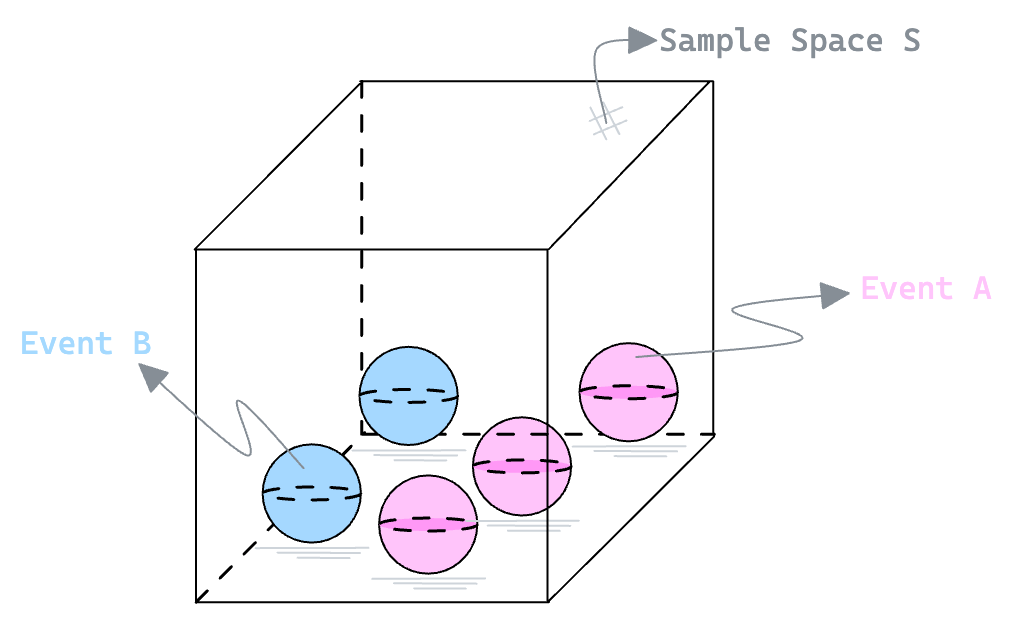
\includegraphics[width=0.5\linewidth]{Figures/sample_space.png}
\caption{Illustration of the sample space as a pebble world, with two events A and B spotlighted}
\label{fig:sample_space}
\end{figure}

\begin{quote}
\setlength{\leftskip}{0.25cm} % Adjust the indentation here
$\color{color2}\Longrightarrow$When the sample space is finite, we can visualize it as a \hlt{pebble world}. Each pebble represents an outcome, and an event is a set of pebbles.
\end{quote}

The table \ref{tab:notation} gives a set of symbols useful when describing events and sets. 

\begin{table}[htbp]
    \centering
    \begin{tabular}{|c|c|}
    \hline
    \textbf{English} & \textbf{Sets} \\
    \hline
    \multicolumn{2}{|c|}{\textbf{Events and occurrences}} \\
    \hline
    sample space & $S$ \\
    \hline
    $s$ is a possible outcome & $s \in S$ \\
    \hline
    $A$ is an event & $A \subseteq S$ \\
    \hline
    $A$ occurred & $s_{\text{actual}} \in A$ \\
    \hline
    something must happen & $s_{\text{actual}} \in S$ \\
    \hline
    \multicolumn{2}{|c|}{\textbf{New events from old events}} \\
    \hline
    $A$ or $B$ (inclusive) & $A \cup B$ \\
    \hline
    $A$ and $B$ & $A \cap B$ \\
    \hline
    not $A$ & $A^c$ \\
    \hline
    $A$ or $B$, but not both & $(A \cap B^c) \cup (A^c \cap B)$ \\
    \hline
    at least one of $A_1, \ldots, A_n$ & $A_1 \cup \ldots \cup A_n$ \\
    \hline
    all of $A_1, \ldots, A_n$ & $A_1 \cap \ldots \cap A_n$ \\
    \hline
    \multicolumn{2}{|c|}{\textbf{Relationships between events}} \\
    \hline
    $A$ implies $B$ & $A \subseteq B$ \\
    \hline
    $A$ and $B$ are mutually exclusive & $A \cap B = \emptyset$ \\
    \hline
    \end{tabular}
    \caption{Sets Symbols Dictionary}
    \label{tab:notation}
\end{table}

\subsection{Naive Definition of Probability}

\begin{definition}
    Let $A$ be an event for an experiment with a finite sample space $S$. The naive probability of $A$ is

    \begin{equation}
    P_{\text{naive}} = \frac{|A|}{|S|} = \frac{\textnormal{number of outcomes favorable to } A}{\textnormal{Total number of outcomes in } S}
    \end{equation}

    here $|\cdot|$ means the size of the sample space.
\end{definition}

The naive definition is very restrictive in that it requires $S$ to e finite, with equal mass for each pebble. 

\subsection{How to Count}

\begin{theorem}[Multiplication Rule]
Consider a compound experiment consisting of two sub-experiments $A$ and $B$. Suppose that Exp $A$ has \hlt{$a$} possible outcomes, and for each of these outcomes Exp $B$ has \hlt{$b$} possible outcomes. Then the compound experiment has $ab$ possible outcomes. 
\end{theorem}

We can see such relation by drawing a \hlt{tree diagram} as the figure \ref{fig:tree_diagram} shows. As we can see we have three ramifications for Exp $A$ and four for Exp $B$. With a total of 12 possible outcomes. Note, that it's often easier to think about the experiments as being in chronological order, but there is no requirements in the multiplication rule that experiment experiment $A$ has to be performed \hlt{before} experiment $B$.

\begin{figure}[ht]
\centering
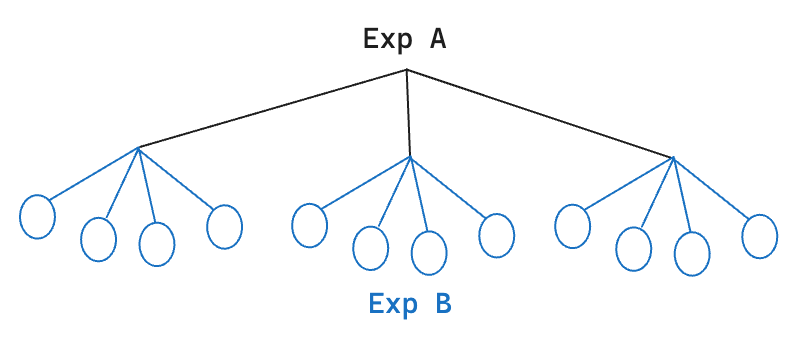
\includegraphics[width=0.5\linewidth]{Figures/tree_diagram.png}
\caption{Tree Diagram.}
\label{fig:tree_diagram}
\end{figure}

\textbf{\underline{Example}}: Suppose that 10 people are participating in a race. Assume that ties are not possible and that all 10 will complete the race, resulting in well-defined first, second, and third place winners. How many possible outcomes are there for these top three positions?

First, there are 10 possible choices for who finishes in first place. After the first place is determined, there remain 9 competitors for the second place, and once both the first and second places are fixed, there are 8 possibilities for the third place. Therefore, by the multiplication rule, the \hlt{total number of possible outcomes} is $10 \cdot 9 \cdot 8 = 720$.

\begin{quote}
\setlength{\leftskip}{0.25cm} % Adjust the indentation here
$\color{color2}\Longrightarrow$ Note that we did not necessarily have to determine the first place winner first. We could have instead considered the third place winner initially, with 10 possibilities, followed by 9 possibilities for the second place, and finally 8 possibilities for the first place. This approach yields the same result, as expected from the multiplication rule.
\end{quote}

Now, let's consider another more common example. Suppose we have a set of 10 unique books and we want to arrange three of them on a shelf. The order of the books matters. How many different arrangements are possible? To solve this, we again use the multiplication rule. We have 10 choices for the first position, 9 choices for the second position, and 8 choices for the third position. Therefore, the total number of different arrangements is $10 \cdot 9 \cdot 8 = 720$.

We can use the multiplication rule to derive formulas for sampling with and without \hlt{replacement}.


\begin{theorem}[\hlti{Sampling with replacement}]
    Consider $n$ objects and making $k$ choices from them, one at a time \hlt{with} \hlt{replacement} (i.e., choosing a certain object does not preclude it from being chosen again). Then there are $n^k$ possible outcomes (where \hlt{order matters}, in the sense that, e.g., choosing object 3 and object 7 is counted as a different outcome than choosing object 7 and object 3).
\end{theorem}

\textbf{\underline{Example}}: Imagine a jar with $n$ balls, labeled from 1 to $n$. We sample balls one at a time with replacement, meaning that each time a ball is chosen, it's returned to the jar. 

By the multiplication rule there are \hlt{$n^k$} ways to obtain a sample of size $k$. We can visualize this in the figure \ref{fig:sampling_replacement}.

\begin{figure}[ht]
\centering
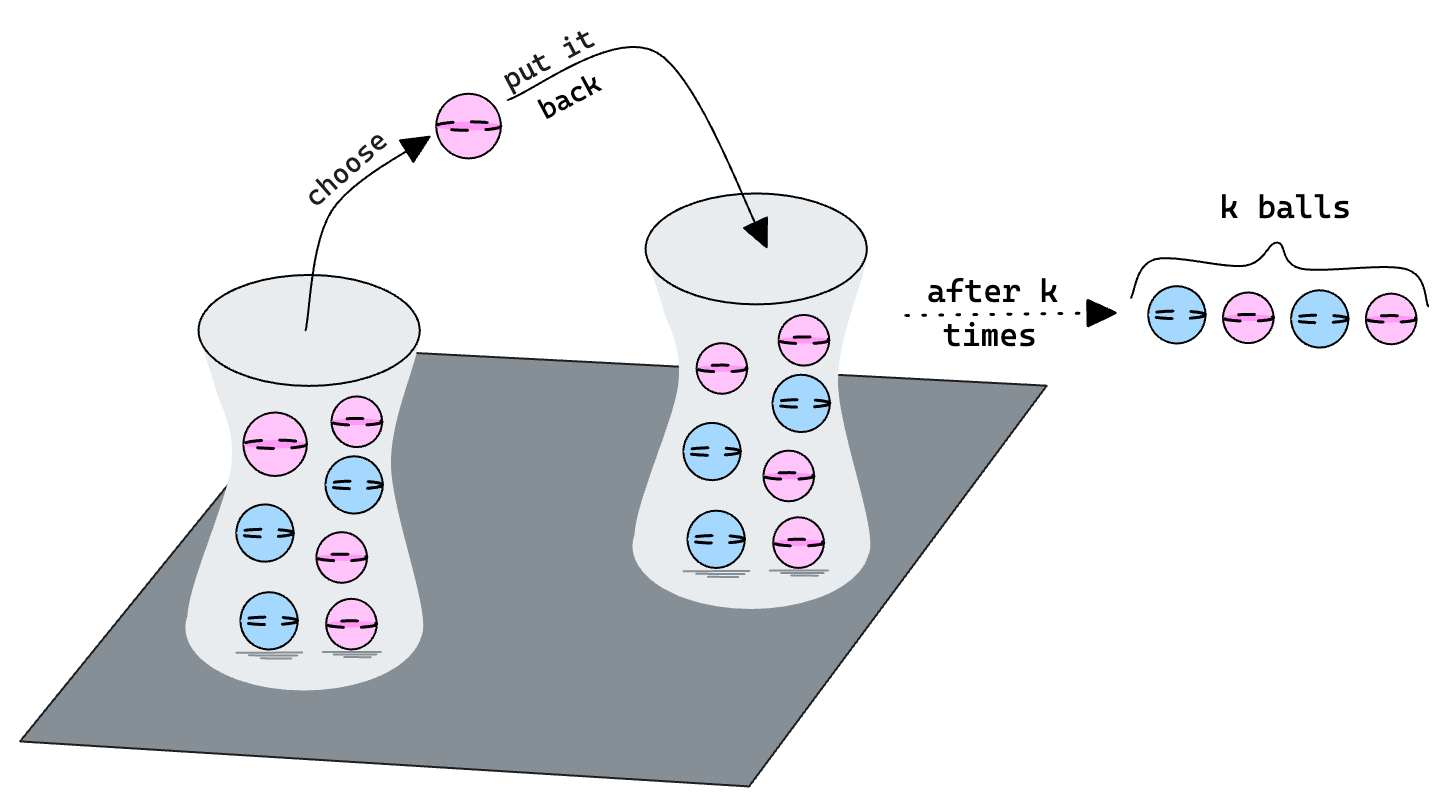
\includegraphics[width=0.6\linewidth]{Figures/sampling_replacement.png}
\caption{Illustration of sampling with replacement.}
\label{fig:sampling_replacement}
\end{figure}

\begin{theorem}[\hlti{Sampling without replacement}]
    Consider $n$ objects and making $k$ choices from them, one at a time without replacement. (i.e., choosing a certain objects precludes it from being chosen again). The there are 

    \begin{equation}
        (n)_k = n(n-1)\cdots(n - k + 1)
    \end{equation}

    possible outcomes for $1 \leq k \leq n$, and 0 possibilities for $k > n$ (where \hlt{order matters}). By convention

    \begin{equation}
        n(n-1)\cdots(n-k+1) = n \textnormal{ for } k = 1
    \end{equation}
\end{theorem}

\begin{quote}
\setlength{\leftskip}{0.25cm} % Adjust the indentation here
$\color{color2}\Longrightarrow$ Special case when $k = n$, $(n)_{k=n} = n!$
\end{quote}

\noindent\textit{\underline{Example:}} There are $k$ people in the room and their birthdays are independent. What is the probability that at least one pair of people in the group have the same birthday?

It's easier to calculate the probability that \hlt{no two people share a birthday}. This amounts to sampling 365 days of the year without replacement.

$$
P(\text{no birthday match}) = \frac{365 \cdot 364 \cdots (365 - k + 1)}{365^k} = P_1
$$

Then,

$$
P(\text{at least 1 birthday match}) = 1 - P_1 = P_2
$$

For $k = 23$ people, $P_2 > 50\%$ and for $k = 57$ people, $P_2 > 99\%$.

\textit{\underline{Example from \cite{feller1}:}} Let the population consist of the ten digits $0, 1, \cdots, 9$. Every succession of five digits represents a sample of size $k = 5$ and we assume that each such arrangement has a probability $p_1 = \frac{1}{10^5} = 10^{-5}$. Then, the \textit{probability $P$ that five consecutive random digits are all different} is

$$
P = \frac{(10)_k}{10^k} = \frac{10 \cdot 9 \cdot 8 \cdot 7 \cdot 6}{10^5} = 0.3024
$$

\subsubsection{"Leibniz mistake"}

\begin{quote}
\setlength{\leftskip}{0.25cm} % Adjust the indentation here
$\color{color2}\Longrightarrow$ It's crucial to think of the objects or people in the population as \hlt{named} or \hlt{labeled}. 
\end{quote}

The "Leibniz mistake" in probability refers to an error made by the mathematician Gottfried Wilhelm Leibniz in the late 17th century regarding the probability of \hlt{mutually exclusive events}.

Leibniz incorrectly calculated the probability of drawing at least one ace from two draws in a deck of cards without replacement. He assumed that the probability of drawing an ace on the first or the second draw could be simply added together, which is only correct for mutually exclusive events. However, these events are not mutually exclusive because drawing an ace on the first draw affects the probability of drawing an ace on the second draw.

Leibniz's mistake was in not accounting for the dependency between the events. The correct calculation should involve conditional probability, which considers the changed probabilities after each draw. This error highlights the importance of understanding the conditions under which probabilities can be directly added, which is a fundamental concept in probability theory.

\subsection{Adjusting for Overcounting}

In many counting problems, it's not easy to directly count each possibility once and only once. However, if we're able to count each possibility exactly $c$ times for some $c$, then we can adjust by dividing by $c$.

\begin{definition}[\hlti{Binomial Coefficient}]
    For any nonnegative integers $k$ and $n$, the binomial coefficient $\binom{n}{k}$, read as \hlt{"n choose k"}, is the number of subsets of size $k$ from a set of size $n$.

    \begin{equation}
        \binom{n}{k} = \frac{n!}{(n - k)! \; k!}
    \end{equation}
\end{definition}

\section{Conditional Probability And Stochastic Independence}

\begin{quote}
\setlength{\leftskip}{0.25cm} % Adjust the indentation here
$\color{color2}\Longrightarrow$ The following subsections were written using the book \cite{feller1} and \textbf{specially} \cite{venkatesh2024} online lectures as references.
\end{quote}

\subsection{Conditional Probability}

Suppose a population of $N$ people includes $N_A$ colorblind people and $N_\mathcal{H}$ females.

$$
p(A) = \frac{N_A}{N} \rightarrow \text{probability of being colorblind} \quad p(\mathcal{H}) = \frac{N_\mathcal{H}}{N} \rightarrow \text{probability of being a female}
$$

We may now restrict our attention to the subpopulation consisting of females. The probability that a person chosen at random from this subpopulation is colorblind equals

$$
P(A | \mathcal{H}) = \frac{N_{A\mathcal{H}}}{N_\mathcal{H}} = \frac{P(A \cap \mathcal{H})}{P(\mathcal{H})}
$$

where $P(A|\mathcal{H})$ is read as "the probability of the event $A$ (colorblindness), assuming the event $\mathcal{H}$ (that the person chosen is female)."

\begin{definition}
    Let $\mathcal{H}$ be an event with positive probability. For an arbitrary event $A$, we shall write
    
    \begin{equation}
     \equationgold{
      P(A|\mathcal{H}) = \frac{P(A \cap \mathcal{H})}{P(\mathcal{H})}
    }
    \end{equation}\\
    
    The quantity so defined will be called the \hlti{conditional probability of $A$ on the hypothesis $\mathcal{H}$} (or for given $\mathcal{H}$). When all sample points have equal probabilities, $P(A|\mathcal{H})$ is the ratio $\frac{N_{A\mathcal{H}}}{N_\mathcal{H}}$ of the number of sample points common to $A$ and $\mathcal{H}$, to the number of points in $\mathcal{H}$.
\end{definition}

Taking conditional probabilities of various events with respect to a \hlt{particular hypothesis} $\mathcal{H}$ amounts to choosing $\mathcal{H}$ as a new sample space with probabilities proportional to the original ones. All general theorems on probabilities are \hlt{valid} also for conditional probabilities with respect to any particular hypothesis $\mathcal{H}$, for instance

\begin{equation}
    P(A \cup B | \mathcal{H}) = P(A | \mathcal{H}) + P(B | \mathcal{H}) - P(A \cap B | \mathcal{H})
\end{equation}

\begin{theorem}[Compound probabilities]
    \begin{equation}
        P(A \cap \mathcal{H}) = P(A | \mathcal{H}) \cdot P(\mathcal{H})
    \end{equation}
\end{theorem}

\noindent\textit{\underline{Example:}} Suppose we have a deck of 52 cards, and we want to find the probability that a randomly drawn card is a king, given that it is a face card (jack, queen, or king). 

Let $A$ be the event "the card is a king," and $\mathcal{H}$ be the event "the card is a face card." There are 12 face cards in total, and 4 of them are kings. The probability that a card is a face card is
$$
P(\mathcal{H}) = \frac{12}{52} = \frac{3}{13}.
$$

The probability that a card is a king and a face card is
$$
P(A \cap \mathcal{H}) = \frac{4}{52} = \frac{1}{13}.
$$

Therefore, the conditional probability that a card is a king given that it is a face card is
$$
P(A | \mathcal{H}) = \frac{P(A \cap \mathcal{H})}{P(\mathcal{H})} = \frac{\frac{1}{13}}{\frac{3}{13}} = \frac{1}{3}.
$$

\noindent\textit{\underline{Example:}} A family with two children is known to have (at least) one boy. What are the chances the other child is also a boy?

Let's consider the following notation:

\begin{itemize}
    \item Let $\mathcal{H}$ be the event of at least one boy
    \item Let $A$ be the event of the other child is also a boy
    \item Let denote our sample space as $\{bb, bg, gb, gg\}$ where $g$ represents a girl and $b$ represents a boy
\end{itemize}

We aim to calculate $P(A | \mathcal{H})$. Thus

$$
    P(bb) = P(bg) = P(gb) = P(gg) = \frac{1}{4}
$$

$$
    P(A | \mathcal{H}) = P(b | b) = \frac{P(A \cap \mathcal{H})}{P(\mathcal{H})} = \frac{P(bb)}{P\{bb, gb, bg\}} = \frac{1/4}{3 \cdot 1/4} \implies P(A | \mathcal{H}) = \frac{1}{3}
$$

\begin{quote}
\setlength{\leftskip}{0.25cm} % Adjust the indentation here
$\color{color2}\Longrightarrow$ Note how our hypothesis space was initially $\{bb, bg, gb, gg\}$ but at the moment we received the information that the family already had \hlt{at least one boy} our hypothesis space changed to $\{bb, bg, gb\}$ nor more $gg$ being considered. This example illustrates, how \hlti{side information} makes the sample space to change. 
\end{quote}

\begin{quote}
\setlength{\leftskip}{0.25cm} % Adjust the indentation here
$\color{color2}\Longrightarrow$ It's interesting that most people expect the answer to be \hlt{1/2}. This is the correct answer to a \hlt{different} question, namely: a boy is chosen at random and found to come from a family with two children; what's the probability that the other child is a boy?
\end{quote}


\begin{definition}[Chain Rule for Conditional Probabilities]
    The chain rule for conditional probabilities states that for any sequence of events $A_1, A_2, \ldots, A_n$, the joint probability of these events can be expressed as the product of conditional probabilities:

    \begin{equation}
        P(A_1 \cap A_2 \cap \cdots \cap A_n) = P(A_1) \cdot P(A_2 | A_1) \cdot P(A_3 | A_1 \cap A_2) \cdots P(A_n | A_1 \cap A_2 \cap \cdots \cap A_{n-1})
    \end{equation}

    This rule allows us to break down the joint probability of a sequence of events into a product of simpler conditional probabilities.
\end{definition}


\noindent\textit{\underline{Example:}} Suppose we want to find the joint probability of three events: $A$, $B$, and $C$. According to the chain rule for conditional probabilities, we can express this as:

$$
P(A \cap B \cap C) = P(A) \cdot P(B | A) \cdot P(C | A \cap B).
$$

Let's consider a specific scenario: drawing three cards sequentially from a standard deck of 52 cards without replacement.

\begin{itemize}
    \item Let $A$ be the event that the first card drawn is an \hlt{Ace}.
    \item Let $B$ be the event that the second card drawn is a \hlt{King}.
    \item Let $C$ be the event that the third card drawn is a \hlt{Queen}.
\end{itemize}

We want to find the probability $ P(A \cap B \cap C) $.

\begin{align*}
    P(A) &= \frac{4}{52} \quad \text{(since there are 4 Aces in a deck of 52 cards)}. \\
    P(B | A) &= \frac{4}{51} \quad \text{(after drawing an Ace, there are 51 cards left, and 4 of them are Kings)}. \\
    P(C | A \cap B) &= \frac{4}{50} \quad \text{(after drawing an Ace and a King, there are 50 cards left, and 4 of them are Queens)}.
\end{align*}

Using the chain rule:

$$
P(A \cap B \cap C) = P(A) \cdot P(B | A) \cdot P(C | A \cap B) = \frac{4}{52} \cdot \frac{4}{51} \cdot \frac{4}{50}.
$$


\begin{theorem}[\hlti{Law of Total Probability}]
    Let $\{\mathcal{H}_j\}$ be a partition of the sample space, meaning that the events $\mathcal{H}_1, \mathcal{H}_2, \ldots, \mathcal{H}_n$ are mutually exclusive and exhaustive (i.e., one of them must occur). Then, for any event $A$,

    \begin{equation}
    \equationgold{
      P(A) = \sum_j P(A \cap \mathcal{H}_j)
    }
    \end{equation}

    Using the definition of conditional probability, we have:

    \begin{equation}
        P(A \cap \mathcal{H}_j) = P(A | \mathcal{H}_j) \cdot P(\mathcal{H}_j).
    \end{equation}

    Substituting this into the equation above, we get:

    \begin{equation}
        P(A) = \sum_j P(A \cap \mathcal{H}_j) = \sum_j P(A | \mathcal{H}_j) \cdot P(\mathcal{H}_j).
    \end{equation}
\end{theorem}

\noindent\textit{\underline{Example:}} Suppose there are two bags, Bag 1 and Bag 2. Bag 1 contains 3 red balls and 7 blue balls, while Bag 2 contains 5 red balls and 5 blue balls. A bag is chosen at random with equal probability, and then a ball is drawn from the chosen bag. We want to find the probability of drawing a red ball.

Let:
\begin{itemize}
    \item $\mathcal{H}_1$ be the event of choosing Bag 1.
    \item $\mathcal{H}_2$ be the event of choosing Bag 2.
    \item $A$ be the event of drawing a red ball.
\end{itemize}

We know:
\begin{align*}
    P(\mathcal{H}_1) &= \frac{1}{2} \quad \text{and} \quad P(\mathcal{H}_2) = \frac{1}{2}. \\
    P(A | \mathcal{H}_1) &= \frac{3}{10} \quad \text{(probability of drawing a red ball from Bag 1)}. \\
    P(A | \mathcal{H}_2) &= \frac{5}{10} \quad \text{(probability of drawing a red ball from Bag 2)}.
\end{align*}

Using the law of total probability:

$$
P(A) = P(A | \mathcal{H}_1) \cdot P(\mathcal{H}_1) + P(A | \mathcal{H}_2) \cdot P(\mathcal{H}_2).
$$

Substituting the values:

$$
P(A) = \left(\frac{3}{10}\right) \cdot \left(\frac{1}{2}\right) + \left(\frac{5}{10}\right) \cdot \left(\frac{1}{2}\right) = \frac{3}{20} + \frac{5}{20} = \frac{8}{20} \implies P(A) = \frac{2}{5}.
$$

So, the probability of drawing a red ball is $ \frac{2}{5} $.

\subsection{Bayes' Rule For Events}

\begin{definition}[Bayes' Rule]
    Given a partition $ \{A_j, j \geq 1\} $ of the sample space $ S $, a \hlt{priori} probabilities $ P(A_j) $, and a forward conditional probability $ P(\mathcal{H} | A_j) $, Bayes' rule states that to determine the \hlt{posterior} probability $ P(A_k | \mathcal{H}) $, we have:

    \begin{equation}
    \equationgold{P(A_k | \mathcal{H}) = \frac{P(\mathcal{H} | A_k) \cdot P(A_k)}{P(\mathcal{H})}}
    \end{equation}
\end{definition}

\begin{equation}
P(\mathcal{H}) = \sum_{j} P(\mathcal{H} | A_j) \cdot P(A_j)
\end{equation}

\begin{equation}
P(A_k \cap \mathcal{H}) = \mathcal{H} | A_k) \cdot P(A_k)
\end{equation}

\noindent Where $\{A_j\}$ are the events that partition $ S $ and

\subsubsection{Intuitive Explanation of Bayes' Rule}

Imagine you are trying to understand the likelihood of a specific event happening based on new information. Bayes' Rule helps you update your beliefs about this event. Here's an intuitive explanation:

\begin{itemize}
    \item \textbf{Prior Belief}: Start with what you already know or believe about the event. This is your \hlt{prior} probability.
    \item \textbf{New Evidence}: You receive \hlt{new information} or evidence related to the event.
    \item \textbf{Likelihood}: Consider how likely this new evidence is if your initial belief (hypothesis) is true.
    \item \textbf{Update Belief}: Adjust your initial belief based on the new evidence. This gives you a new, updated probability, called the \hlt{posterior} probability.
\end{itemize}

In simpler terms, Bayes' Rule allows you to refine your initial assumptions (prior beliefs) by incorporating new data (evidence) to get a more accurate understanding (posterior belief) of the event's likelihood. It's like revising your opinion about something after considering \hlti{additional information}. There are two schematics that help me a lot in understanding how Bayes' Rule is computed. Please refer to Figure \ref{fig:bayes_schematic}. 

\begin{figure}[ht]
\centering
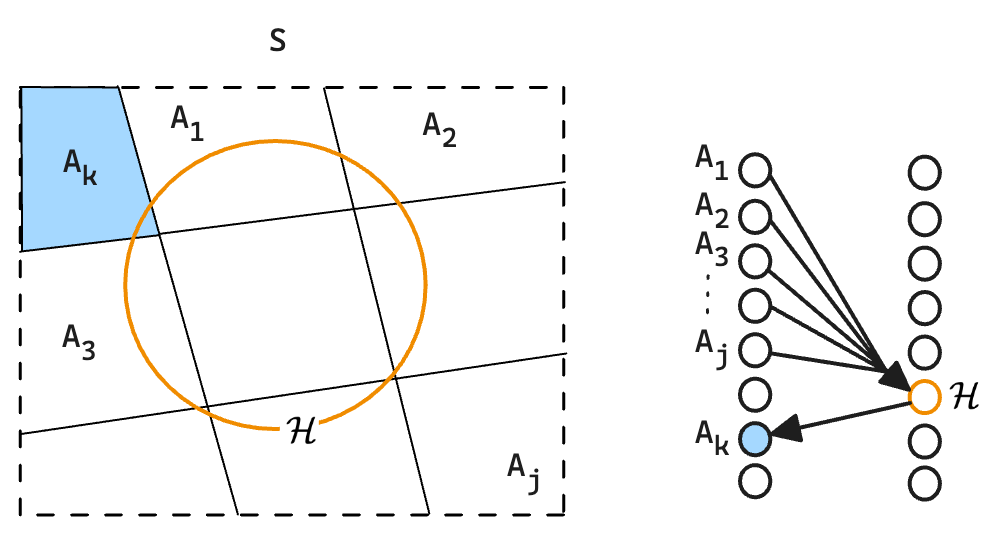
\includegraphics[width=0.4\linewidth]{Figures/bayes_schematic.png}
\caption{Illustration of how to understand Bayes' formula.}
\label{fig:bayes_schematic}
\end{figure}

\begin{itemize}
    \item \textbf{Left Diagram}: The sample space $ S $ is partitioned into several events $ \{A_1, A_2, A_3, \ldots, A_j\} $. Each of these events represents a possible state or outcome. The event $ A_k $ is highlighted in blue, indicating the specific event for which we want to determine the posterior probability given the hypothesis $ \mathcal{H} $, which is represented by the orange circle. The goal is to calculate the probability of $ A_k $ given $ \mathcal{H} $, denoted as $ P(A_k | \mathcal{H}) $.

    \item \textbf{Right Diagram}: This diagram represents the flow of information between events and the hypothesis. Each event $ A_j $ (with $ j \geq 1 $) has a direct influence on the hypothesis $ \mathcal{H} $. The highlighted event $ A_k $ (in blue) directly contributes to the hypothesis. The arrows indicate the direction of conditional dependencies. We start with the prior probabilities $ P(A_j) $ and the conditional probabilities $ P(\mathcal{H} | A_j) $, and use Bayes' rule to update our belief about $ A_k $ given the occurrence of $ \mathcal{H} $.

    The key idea is to combine our prior belief about the events (left diagram) with new evidence (right diagram) to update our understanding of the specific event $ A_k $ in the context of the hypothesis $ \mathcal{H} $.
\end{itemize}

\subsubsection{Side information}

One might believe that side information always increases the probability being calculated. However, conditioning provides information that can affect event probabilities in \hlti{unexpected} ways.\\

\noindent\textit{\underline{Example:}} Suppose we have a test for a rare disease that affects 1 in 1,000 people. The test is 99\% accurate for those with the disease (true positive rate) and 99\% accurate for those without the disease (true negative rate). If a person tests positive, what is the probability that they actually have the disease?

Let:
\begin{itemize}
    \item $D$ be the event that the person has the disease and $D^c$ the event that the person doesn't have the disease.
    \item $T^+$ be the event that the person tests positive.
\end{itemize}

We know:
\begin{align*}
    P(D) &= \frac{1}{1000} \quad \text{(prior probability of having the disease)}. \\
    P(T^+ | D) &= 0.99 \quad \text{(probability of testing positive given the disease)}. \\
    P(T^+ | D^c) &= 0.01 \quad \text{(probability of testing positive given no disease)}. \\
    P(D^c) &= 1 - P(D) = \frac{999}{1000} \quad \text{(\hlt{prior} probability of not having the disease)}.
\end{align*}

We know from our conditional probability definition that

$$
P(A | \mathcal{H}) = \frac{P(A \cap \mathcal{H})}{P(\mathcal{H})}
$$

\noindent applying this to our problem, our hypothesis is that the person tests positive, represented as $P(\mathcal{H}) = P(T^+)$, and we want to calculate the probability that they actually have the disease \hlt{given} that their test result is positive. In other words, we aim to find $P(D | T^+)$, thus
$$
P(D | T^+) = \frac{P(D) \cap P(T^+)}{P(T^+)} = \frac{P(T^+ | D) \cdot P(D)}{P(T^+)}
$$

Where
$$
P(T^+) = P(T^+ | D) \cdot P(D) + P(T^+ | D^c) \cdot P(D^c).
$$

Substituting the values:
\begin{align*}
    P(T^+) = (0.99) \cdot \left(\frac{1}{1000}\right) + (0.01) \cdot \left(\frac{999}{1000}\right) = \frac{0.99}{1000} + \frac{9.99}{1000} = \frac{10.98}{1000} \implies P(T^+) = 0.01098.
\end{align*}

Therefore,
\begin{align*}
    P(D | T^+) = \frac{0.99 \cdot \frac{1}{1000}}{0.01098} = \frac{0.00099}{0.01098} \implies P(D | T^+) = 0.0902 = 9.02\%.
\end{align*}

So, the probability that a person actually has the disease given a positive test result is approximately 9.02\%, illustrating how conditioning on additional information can yield surprising results.

\section{Introduction to Information Theory}

\begin{quote}
\setlength{\leftskip}{0.25cm} % Adjust the indentation here
$\color{color2}\Longrightarrow$ The following section was written using the book \cite{mackay_book} and \cite{mackay_youtube_playlist} online lectures as references.
\end{quote}

\subsection{How can we achieve perfect communication over an imperfect, noisy communication channel?}

\noindent \underline{\textit{Example:}} Imagine you are playing a game of telephone, where one person whispers a message to the next person, and so on. Each person transmits the message correctly with a probability of $ (1 - p) $ and incorrectly with a probability of $ p $.

Let's denote:
\begin{itemize}
    \item $ p $: The probability of transmitting the message incorrectly.
    \item $ (1 - p) $: The probability of transmitting the message correctly.
    \item $ n $: The number of people the message is passed through.
\end{itemize}

The \hlt{binary symmetric channel} model can be used to analyze this scenario. The probability that the message is received incorrectly after being passed through $ n $ people can be calculated as follows:

\begin{equation}
P(\text{error}) = 1 - (1 - p)^n
\end{equation}

This formula assumes that each person makes an independent error with probability $ p $. For example, if the message is passed through 3 people and each person has a 10\% chance of making an error, the probability that the message is received incorrectly is:

\begin{equation}
P(\text{error}) = 1 - (1 - 0.1)^3 = 1 - 0.9^3 \approx 0.271
\end{equation}

Thus, there is approximately a 27.1\% chance that the message will be incorrect after being passed through 3 people.

The figure \ref{fig:bsc} shows how the Binary Symmetric Channel (BSC) can be visualized. It can basically me understood as a communication channel that follows the Binomial Distribution. 

\begin{quote}
\setlength{\leftskip}{0.25cm} % Adjust the indentation here
$\color{color2}\Longrightarrow$ For a \hlt{binomial} distribution, the \hlt{mean} is given by $Np$ and the \hlt{variance} is $Npq = \sigma^2$.
\end{quote}

\begin{figure}[ht]
\centering
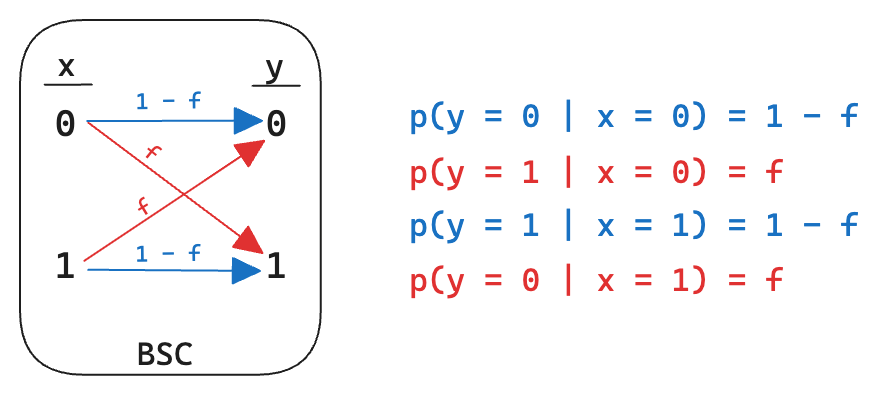
\includegraphics[width=0.6\linewidth]{Figures/bsc.png}
\caption{Binary Symmetric Channel (BSC)}
\label{fig:bsc}
\end{figure}



\subsubsection{What do we mean by \emph{channel}?}

Figure \ref{fig:encoder_schematic} illustrates the basic concept of transmitting a message. We start with a source message $ S $ that needs to be encoded before transmission. For example, when speaking to someone, we encode our ideas into a form that can be transmitted, and the listener must understand this encoding process to decode the message. For instance, if we are speaking in English, the English language serves as the encoding method for our source message. After encoding the message, we use our voice to transmit it, typically through the air channel in a normal conversation or through a call. The listener then needs to decode the message by understanding how to convert the sounds we make with our mouth into meaningful messages. This is, of course, a simplified view of the process of encoding, transmitting, and decoding a message. 

However, during this process of communication, something might happen that introduces sufficient noise to the point where the other person cannot understand what we intended to say. With that in mind, we wonder: is there a way to correct these errors? And if there is, \textit{what is the \hlt{best error-correcting} performance we can achieve?}

\begin{figure}[ht]
\centering
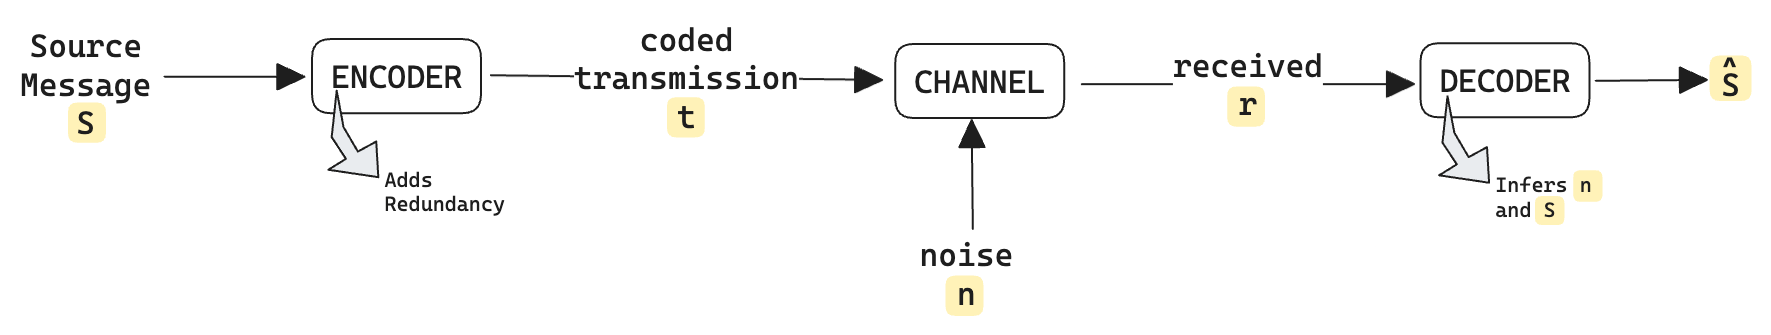
\includegraphics[width=\linewidth]{Figures/encoder_schematic.png}
\caption{Process of the Encoding of a Message}
\label{fig:encoder_schematic}
\end{figure}

Let's see some practical examples of why correcting communication errors is very important.\\

\noindent \underline{\textit{Example:}} Imagine we want to buy a flash drive. However, the flash drive has a problem. Every bit you send to it to be saved will sometimes be flipped. Let's suppose that your large .mp3 file has a chunk of bits like $0011100\cdots$, and you transfer this .mp3 file to be saved on this flash drive. But the flash drive makes an error and saves it as $0011101\cdots$. The manufacturer of the drive says that around 10\% of the bits will be flipped when saving files. How worried should we be if we're buying this flash drive?\\


Let's imagine our .mp3 file has $N = 10,000$ bits which we need to store in the flash drive. Based on the manufacturer's information, the probability of error is given by $f = 0.1$. We can model this process of saving our file as a Binary Symmetric Channel, as shown in Figure \ref{fig:bsc}. Thus, if we send a bit $x = 1$ to be saved on the flash drive, but a zero is saved $y = 0$, we can express this probability as $P(y = 0 | x = 1) = f$. This reads as, \textit{given that we have transmitted a 1, what's the probability we receive a zero}?

With that in mind, how can we calculate the total number of bits flipped if we try to save a file with $N = 10,000$ bits? As we've seen, the Binary Symmetric Channel (BSC) can be modeled as a binomial distribution, and we know that the mean or expected value of a binomial distribution is given by $E[X] = Np$. So, what is the expected number of bits to be flipped by this flash drive?

$$
E[X] = 10,000 \cdot f = 1,000
$$

This means that around 1,000 bits will be saved incorrectly. However, for a more precise estimate, we should also consider the standard deviation $\sigma$, which for a binomial distribution is calculated as $\sigma = \sqrt{Var[X]} = \sqrt{Npq}$.

$$
Var[X] = 10,000 \cdot 0.1 \cdot 0.9 = 900 \implies \sigma = \sqrt{900} = 30
$$

Finally, the number of bits flipped can be expressed as:

$$  
\text{Number of bits flipped} = Np \pm \sqrt{Npq} = 1,000 \pm 30
$$

Therefore, we should be a bit worried :(\\

\subsubsection{Adding Redundancy}

\noindent \underline{\textit{Example:}} How can we help the flash drive company correct this saving malfunction?\\

The keyword here is \hlti{redundancy}. We want our encoders to add \textit{redundancy}. This way, if our flash drive makes a mistake, we can try to check if an error occurred. Remember, sometimes we don't have access to the original transmitted file or message. We need to be clever in this approach.

Let's analyze two simple strategies we could employ to fix add redundancy to the encoding process. 

\begin{enumerate}
    \item \hlti{\textbf{Parity Encoding}}: Imagine we receive the bits $10101$. We could append one extra bit at the end of every message to indicate whether we have an even or odd quantity of bits. For instance, $10101$ would have a $parity = 1$ because there are three ones (odd). Similarly, $11110$ would have a $parity = 0$ because there are four ones (even). This way, if we receive a message with an even number of ones but the parity bit is 1, we can be certain that an error occurred when saving this file. However, with parity coding, as you have probably noticed, we can only detect errors, not correct them :/

    \item \hlti{\textbf{Repetition Code}}: Repetition codes are a simple form of error detection and correction. The idea is to repeat each bit of the message multiple times. For instance, if we want to transmit the bit `1', we might repeat it three times, sending `111'. Similarly, to transmit the bit `0', we would send `000'. When the receiver gets the message, they use a \hlt{majority vote} to determine the original bit. For example, if the receiver gets `110', they would interpret it as `1' because the majority of the bits are `1'. This method helps to correct errors as long as the number of errors is less than half the number of repetitions.
\end{enumerate}

Let's imagine we receive a file with three bits, and we wish to use the repetition code to make it work. Thus, let's understand the table \ref{tab:likelihood_decoding}. It shows the received sequences $r$, their likelihood ratios $\frac{P(r|s=1)}{P(r|s=0)}$, and the decoded sequences $\hat{s}$. The decoding algorithm assumes the channel is a binary symmetric channel with $\gamma = \frac{(1 - f)}{f}$, where $f$ is the error probability.

\begin{table}[h!]
    \centering
    \begin{tabular}{cccc}
        \hline
        Received sequence $r$ & Likelihood ratio $\frac{P(r|s=1)}{P(r|s=0)}$ & Decoded sequence $\hat{s}$ \\
        \hline
        000 & $\gamma^{-3}$ & 0 \\
        001 & $\gamma^{-1}$ & 0 \\
        010 & $\gamma^{-1}$ & 0 \\
        100 & $\gamma^{-1}$ & 0 \\
        101 & $\gamma^{1}$ & 1 \\
        110 & $\gamma^{1}$ & 1 \\
        011 & $\gamma^{1}$ & 1 \\
        111 & $\gamma^{3}$ & 1 \\
        \hline
    \end{tabular}
    \caption{Likelihood ratios and decoded sequences for a binary symmetric channel \cite{mackay_book}.}
    \label{tab:likelihood_decoding}
\end{table}

To explain the \hlt{optimal decoding decision} (i.e., the decision that minimizes the probability of being wrong), we need to find the value of $s$ that is most probable, given $r$.  Consider the decoding of a single bit $s$, which was encoded as the sequence $r = r_1 r_2 r_3$. By Bayes' theorem, the posterior probability of $s$ is:

\begin{equation}
P(s|r_1 r_2 r_3) = \frac{P(r_1 r_2 r_3|s) P(s)}{P(r_1 r_2 r_3)}
\end{equation}

We can spell out the posterior probabilities of the two alternatives thus:

\begin{equation}
P(s=1|r_1 r_2 r_3) = \frac{P(r_1 r_2 r_3|s=1) P(s=1)}{P(r_1 r_2 r_3)}
\end{equation}

\begin{equation}
P(s=0|r_1 r_2 r_3) = \frac{P(r_1 r_2 r_3|s=0) P(s=0)}{P(r_1 r_2 r_3)}
\end{equation}

The posterior probability is determined by two factors: the \hlt{prior} probability $P(s)$ and the \hlt{data-dependent} term $P(r_1 r_2 r_3|s)$, which is called the \hlt{likelihood} of $s$. Assuming the prior probabilities are equal ($P(s=0) = P(s=1) = 0.5$), then maximizing the posterior probability $P(s|r)$ is equivalent to \hlt{maximizing} the likelihood $P(\bm{r}|s)$. 

Assuming the channel is a binary symmetric channel with noise level $f < 0.5$, which in our case for the flash drive manufacturer is $f = 0.1$, the likelihood is:

\begin{equation}
P(\bm{r}|s) = P(\bm{r}|t(s)) = \prod_{n=1}^{N} P(r_n | t_n(s))
\end{equation}

\noindent where $N = 3$ is the \hlt{number of transmitted bits in the block}, and:

\begin{equation}
P(r_n | t_n) = 
\begin{cases} 
(1 - f) & \text{if } r_n = t_n \\ 
f & \text{if } r_n \neq t_n 
\end{cases}
\end{equation}

Thus, the likelihood ratio for the two hypotheses is:

\begin{equation}
\frac{P(r|s=1)}{P(r|s=0)} = \prod_{n=1}^{N} \frac{P(r_n | t_n(1))}{P(r_n | t_n(0))}
\end{equation}

Each factor $\frac{P(r_n | t_n(1))}{P(r_n | t_n(0))}$ equals $\left(\frac{1-f}{f}\right)$ if $r_n = 1$ and $\left(\frac{f}{1-f}\right)$ if $r_n = 0$. The ratio 

$$
\gamma = \left(\frac{1-f}{f}\right)
$$

\noindent implies that the winning hypothesis is the one with the most `votes', each \hlt{vote counting for a factor of $\gamma$} in the likelihood ratio. 

Thus, the majority-vote decoder shown in table \ref{tab:likelihood_decoding} is the \hlt{optimal} decoder if we assume that the channel is a binary symmetric channel and that the two possible values of $s$ are equally likely. For a more in depth explanation please refer to \cite{mackay_book}.


\begin{quote}
\setlength{\leftskip}{0.25cm} % Adjust the indentation here
$\color{color2}\Longrightarrow$ If we use repetition code to communicate data over a telephone line for example, it'll \hlt{reduce} the error frequency, but it'll also reduce our communication rate. We'll have to \hlt{pay three times} as much for each phone call.
\end{quote}

\section{Markov Chains and Information Source}

\begin{quote}
\setlength{\leftskip}{0.25cm} % Adjust the indentation here
$\color{color2}\Longrightarrow$ The following sections used the following books as reference \cite{mackay_book, feller1}
\end{quote}

Independent trials can be described as a set of possible outcomes where $E_1, E_2, \cdots$ (finite or infinite in number) is given, and with each there's associated a probability $P_k$; the probabilities of sample sequences are defined by the multiplicative property

\begin{equation}
    P\{ (E_{j0}, E_{j1}, \cdots, E_{jn})\} = P_{j0}P_{j1} \cdots P_{jn}
\end{equation}

\begin{quote}
\setlength{\leftskip}{0.25cm} % Adjust the indentation here
$\color{color2}\Longrightarrow$ In the theory of Markov chains, we consider the simplest generalization which consists in permitting the outcome of any trial to depend on the outcome of the directly preceding trial (\hlti{and only on it}).
\end{quote}

The outcome $E_k$ is no longer associated with a fixed probability $P_k$, but to every pair $(E_j, E_k)$ there corresponds a conditional probability $P_{jk}$; given that $E_j$ has occurred at some trial, the probability of $E_k$ at the next trial is $P_{jk}$. In addition to $P_{jk}$, we must be given the probability \hlt{$a_k$} of the outcome $E_k$ of the initial trial. For $P_{jk}$ to have the meaning attributed to them, the probabilities of sample sequences corresponding to two trials are

$$
P\{ (E_{j}, E_{k})\}  = a_k P_{jk}
$$

For three trials:
$$
P\{ (E_{j}, E_{k}, E_{r})\}  = a_k P_{jk} P_{kr}
$$

For four trials:
$$
P\{ (E_{j}, E_{k}, E_{r}, E_{s})\}  = a_k P_{jk} P_{kr} P_{rs}
$$

And generally we have:
\begin{equation}
    \equationgold{
    P\{ (E_{j0}, E_{j1}, \cdots, E_{jn}) \} = a_{j0}P_{j0j1}P_{j1j2} \cdots P_{j_{n-2}j_{n-1}}P_{j_{n-1}j_n}
    }
\end{equation}

A sequence of trials with possible outcomes $E_1, E_2, \cdots$ is called a Markov chain if the probabilities of sample sequences are defined by the equation above in terms of a probability distribution $\{ a_k \}$ for each $E_k$ at the initial (or zero-th) trial and fixed conditional probabilities $P_{jk}$ of $E_k$ given that $E_j$ has occurred at the preceding trial.

\begin{quote}
\setlength{\leftskip}{0.25cm} % Adjust the indentation here
$\color{color2}\Longrightarrow$ $P_{jk}$ is called the \hlt{probability of a transition} from $E_j$ to $E_k$ given by $P(X_{t + 1} = j | X_t = k) = p_{jk}$.
\end{quote}

We can compute a \hlt{matrix of transition probabilities} as shown below, which gives us the probability of changing each state.

$$
P = \begin{bmatrix}
p_{11} & p_{12} & \cdots & p_{1k} & \cdots & p_{1n} \\
p_{21} & p_{22} & \cdots & p_{2k} & \cdots & p_{2n} \\
\vdots & \vdots & \ddots & \vdots & \ddots & \vdots \\
p_{j1} & p_{j2} & \cdots & p_{jk} & \cdots & p_{jn} \\
\vdots & \vdots & \ddots & \vdots & \ddots & \vdots \\
p_{n1} & p_{n2} & \cdots & p_{nk} & \cdots & p_{nn} \\
\end{bmatrix}
$$


\begin{definition}
    A stochastic process is said to be \textbf{stationary} if the joint distribution of any subset of the sequence of random variables is invariant with respect to shifts in the time index; that is,

    \begin{equation}
        Pr\{ X_1 = x_1, X_2 = x_2, \cdots, X_n = x_n \} = Pr\{ X_{1 + l} = x_1, X_{2 + l} = x_2, \cdots, X_{n + l} = x_n \}
    \end{equation}

    For every $n$ and every shift $l$ and for all $x_1, x_2, \cdots, x_n \in \mathcal{X}$.
\end{definition}

\subsubsection{Markov Information Source}

This is a source of information that allows the probability distribution of the output at any point in time to be determined in a fixed manner from only the $m$ outputs immediately before that point, regardless of the previous outputs. More formally, for random variables $X_1, X_2, \cdots X_n$, where $n\geq3$, $X_1 \rightarrow X_2 \rightarrow \cdots \rightarrow X_n$ forms a Markov chain if 

\begin{equation}
    P(x_1, x_2, \cdots, x_n)P(x_2)P(x_3) \cdots P(x_{n-1}) = P(x_1, x_2)P(x_2, x_3) \cdots P(x_{n-1}, x_n)
\end{equation}

For all $x_1, x_2, \cdots, x_n$, or equivalently

\begin{align}
    P(x_1, x_2, \cdots, x_n) = P(x_1, x_2)P(x_3 | x_2)\cdots P(x_n | x_{n-1}) \text{ if } P(x_2), P(x_3), \cdots, P(x_{n-1}) > 0 \text{ and 0 otherwise.}
\end{align}

Or we could define it as:

\begin{equation}
    \equationgold{
    P_{X_i | X_{i-1} \cdots X_{i - n}}(x_i | x_{i-1}, \cdots, x_{i-n}) = P_{X_i | X_{i - 1}, \cdots, X_{i-m}}(x_i | x_{i-1}, \cdots, x_{i-m}) \text{ for } n \geq m
    }
\end{equation}

\subsubsection{Stationary Distributions}

\begin{quote}
\setlength{\leftskip}{0.25cm} % Adjust the indentation here
$\color{color2}\Longrightarrow$ This subsection used the following tutorial as reference \cite{stationary_distributions}
\end{quote}

\textit{What's the probability of making a transition from state $i$ to state $j$ over \textbf{two} steps?}

\begin{align*}
    P(X_2 = j | X_0 = i) &= \sum_{k=1}^{N}P_i(X_2 = j | X_1 = k)P_i(X_1 = k) = \sum_{k=1}^{N}P(X_2 = j | X_1 = k, X_0 = i)P(X_1 = k | X_0 = i)\\
    P(X_2 = j | X_0 = i) &= \sum_{k=1}^{N}P(X_2 = j | X_1 = k)P(X_1 = k | X_0 = i)\\
    P(X_2 = j | X_0 = i) &= \sum_{k=1}^{N}p_{kj}p_{ik}\\
    P(X_2 = j | X_0 = i) &= \sum_{k=1}^{N}p_{ik}p_{kj} = (P^2)_{ij} \text{, where $P$ is the transition matrix.}
\end{align*}

Thus we can represent our possible states using the following matrix $\pi$,

$$
\pi = 
\begin{bmatrix}
P(X_0 = s_1) \\
P(X_0 = s_2) \\
\vdots \\
P(X_0 = s_N)
\end{bmatrix}
=
\begin{bmatrix}
\pi_1 \\
\pi_2 \\
\vdots \\
\pi_N
\end{bmatrix}
$$

With that in mind, let $\{X_n\}$ be a Markov chain on $S$ with transition probability matrix $P$. A distribution $\pi$ on $S$ is called stationary (or invariant) if


\begin{equation}
    \equationgold{
        \pi = \pi P    
    }
\end{equation}

or equivalently if

\begin{equation}
    \equationgold{
        \pi_j = \sum_{i \in S} \pi_i p_{ij}, \quad j \in S
    }
\end{equation}

Thus, in order to find a stationary distribution of a Markov chain with a transition probability matrix $P = [p_{ij}]$, we need to solve the linear system (6.1) (or equivalently (6.2)) together with the conditions:
$$
\sum_{i} \pi_i = 1 \quad \text{and} \quad \pi_i \geq 0 \text{ for all } i \in S.
$$\\

\noindent \textit{\underline{Example:}} \textbf{2-state Markov chain}. Consider the transition matrix:

$$
P = \begin{bmatrix}
1 - p & p \\
q & 1 - q
\end{bmatrix}.
$$
Solving the equation $\pi P = \pi, \pi = [\pi_0 \, \pi_1]$, which is equivalent to $\pi_0 p + \pi_1 q = 0$, together with $\pi_0 + \pi_1 = 1$, we obtain

$$
\pi_0 = \frac{q}{p + q}, \quad \pi_1 = \frac{p}{p + q}
$$

\noindent Thus we conclude:
\begin{itemize}
    \item[(i)] If $p + q > 0$, there exists a unique stationary distribution.
    \item[(ii)] If $p = q = 0$, a stationary distribution is not uniquely determined. In fact, any distribution $\pi = [\pi_0, \pi_1]$ is stationary.\\
\end{itemize}

\noindent \underline{\textit{Example:}} A particle moves along the $x$-axis in such a way that its absolute speed remains constant but the direction of the motion can be reversed. The system is said to be in state $E_1$ if the particle moves in the positive direction, and in state $E_2$ if the motion is to the left. Let's denote

\begin{itemize}
    \item $\alpha \rightarrow$ probability of reversal when the particle moves to the right 
    \item $\beta \rightarrow$ probability of reversal when the particle moves to the left 
\end{itemize}

Given the transition matrix shown below and the transition diagram in Figure \ref{fig:two_state_markov}, we can solve this problem by using the stationary equation $\pi = \pi P$, where $\pi = [\pi_0, \pi_1]$. That is

$$
[\pi_0 \ \pi_1] \begin{bmatrix}
1 - \alpha & \alpha \\
\beta & 1 - \beta 
\end{bmatrix} = [\pi_0, \pi_1]
$$

\begin{figure}[ht]
\centering
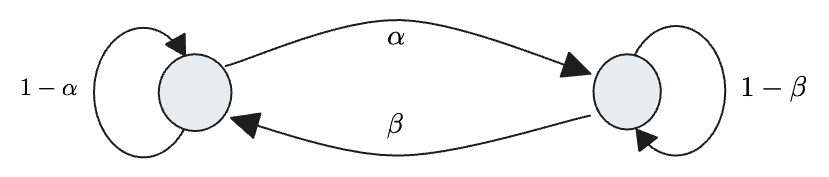
\includegraphics[width=0.6\linewidth]{Figures/two_state_markov.png}
\caption{Two State Markov Chain}
\label{fig:two_state_markov}
\end{figure}

This implies the system of equations:

$$
\pi_0(1 - \alpha) + \pi_1 \beta = \pi_0 \quad \text{and} \quad \pi_0 \alpha + \pi_1(1 - \beta) = \pi_1
$$

and we know that $\sum_i \pi_i = 1 \implies \pi_0 + \pi_1 = 1$. Thus,

$$
\pi_0(1 - \alpha) + \beta(1 - \pi_0) = \pi_0 \implies \pi_0 - \alpha \pi_0 + \beta - \beta \pi_0 = \pi_0 \implies \pi_0 = \frac{\beta}{\alpha + \beta}
$$

Similarly,

$$
(1 - \pi_1)\alpha + \pi_1(1 - \beta) = \pi_1 \implies \pi_1 = \frac{\alpha}{\alpha + \beta}
$$

By setting $\alpha = 0.3$ and $\beta = 0.2$, we created an animation and code that can be executed using the following \href{https://github.com/igor17400/information-theory-174/blob/main/notebooks/markov.ipynb}{link}. Additionally, we included Figure \ref{fig:markov_example_1}, which illustrates the particle movements at each step based on the stationary equations we derived for $\pi_0$ and $\pi_1$.

\begin{figure}[ht]
    \centering
    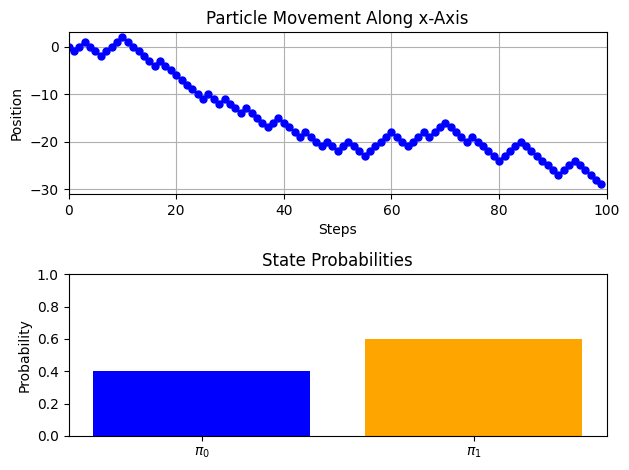
\includegraphics[width=0.6\linewidth]{Figures/markov_example_1.png}
    \caption{Particle movement with markov chains}
    \label{fig:markov_example_1}
\end{figure}


\noindent \underline{\textit{Example:}} A user moves among four different places: Home, Work, Park, and Bar. The system is said to be in state $E_i$ if the user is at place $i$, where $i \in \{\text{Home, Work, Park, Bar}\}$. Let's denote:

\begin{itemize}
    \item $p_{ij} \rightarrow$ probability of moving from place $i$ to place $j$
\end{itemize}

Given the transition matrix shown below and the transition diagram, we can solve this problem by using the stationary equation $\pi = \pi P$, where $\pi = [\pi_0, \pi_1, \pi_2, \pi_3]$. That is,

$$
\pi = [\pi_{\text{Home}} \ \pi_{\text{Work}} \ \pi_{\text{Park}} \ \pi_{\text{Bar}}]
$$

and

$$
P = \begin{bmatrix}
0.5 & 0.3 & 0.1 & 0.1 \\ 
0.2 & 0.5 & 0.2 & 0.1 \\ 
0.3 & 0.3 & 0.3 & 0.1 \\ 
0.2 & 0.3 & 0.2 & 0.3
\end{bmatrix}.
$$

This implies the system of equations:

$$
\pi_{\text{Home}}(0.5) + \pi_{\text{Work}}(0.2) + \pi_{\text{Park}}(0.3) + \pi_{\text{Bar}}(0.2) = \pi_{\text{Home}}
$$
$$
\pi_{\text{Home}}(0.3) + \pi_{\text{Work}}(0.5) + \pi_{\text{Park}}(0.3) + \pi_{\text{Bar}}(0.3) = \pi_{\text{Work}}
$$
$$
\pi_{\text{Home}}(0.1) + \pi_{\text{Work}}(0.2) + \pi_{\text{Park}}(0.3) + \pi_{\text{Bar}}(0.2) = \pi_{\text{Park}}
$$
$$
\pi_{\text{Home}}(0.1) + \pi_{\text{Work}}(0.1) + \pi_{\text{Park}}(0.1) + \pi_{\text{Bar}}(0.3) = \pi_{\text{Bar}}
$$

and we know that $\sum_i \pi_i = 1 \implies \pi_{\text{Home}} + \pi_{\text{Work}} + \pi_{\text{Park}} + \pi_{\text{Bar}} = 1$. Thus,

$$
\begin{aligned}
&\pi_{\text{Home}}(0.5) + \pi_{\text{Work}}(0.2) + \pi_{\text{Park}}(0.3) + \pi_{\text{Bar}}(0.2) = \pi_{\text{Home}} \\
&\pi_{\text{Home}}(0.3) + \pi_{\text{Work}}(0.5) + \pi_{\text{Park}}(0.3) + \pi_{\text{Bar}}(0.3) = \pi_{\text{Work}} \\
&\pi_{\text{Home}}(0.1) + \pi_{\text{Work}}(0.2) + \pi_{\text{Park}}(0.3) + \pi_{\text{Bar}}(0.2) = \pi_{\text{Park}} \\
&\pi_{\text{Home}}(0.1) + \pi_{\text{Work}}(0.1) + \pi_{\text{Park}}(0.1) + \pi_{\text{Bar}}(0.3) = \pi_{\text{Bar}} \\
&\pi_{\text{Home}} + \pi_{\text{Work}} + \pi_{\text{Park}} + \pi_{\text{Bar}} = 1
\end{aligned}
$$

Solving these equations, we find the stationary distribution $\pi$. Using a Python script available at this \href{https://github.com/igor17400/information-theory-174/blob/main/notebooks/markov.ipynb}{link}, we can visualize the evolution of state probabilities over time, showing how the user's location probabilities change with each step in the Markov chain. Figure \ref{fig:markov_example_2} illustrates the likelihood of the user being in each of the four states (Home, Work, Park, Bar) at any given step.

\begin{figure}[ht]
    \centering
    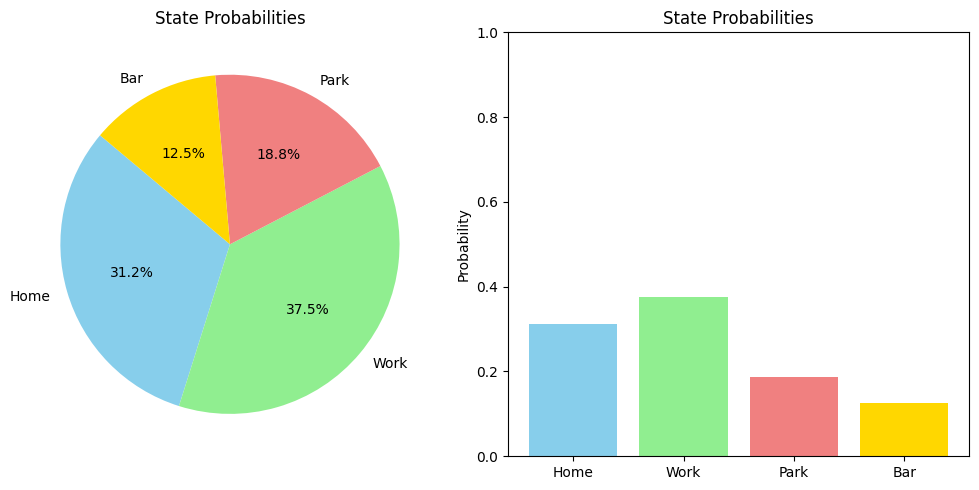
\includegraphics[width=0.6\linewidth]{Figures/markov_example_2.png}
    \caption{Likelihood of the user being in each of the four states (Home, Work, Park, Bar) at any given step.}
    \label{fig:markov_example_2}
\end{figure}

\begin{quote}
    \setlength{\leftskip}{0.25cm} % Adjust the indentation here
    $\color{color2}\Longrightarrow$ I recommend watching the following video \cite{Sachdeva_MarkovChains} for an explanation and visual animations for Markov Chains. 
\end{quote}

\section{Entropy, Relative Entropy, and Mutual Information}

\begin{quote}
\setlength{\leftskip}{0.25cm} % Adjust the indentation here
$\color{color2}\Longrightarrow$ The following section was written using mainly the book \cite{willey_info_theory} as references.
\end{quote}

\subsection{Entropy}

Let $X$ be a discrete random variable with alphabet $\mathcal{X}$ and probability mass function $P(x) = P\{ X = x \}, x \in \mathcal{X}$. We denote the probability mass function by $p(x)$ rather than $P_X(x)$.

\begin{definition}
    The \hlt{entropy} $H(X)$ of a discrete random variable $X$ is defined by 
    \begin{equation}
        \equationgold{
            H(X) = - \sum_{x \in \mathcal{X}} p(x)\log(p(x))
        }
    \end{equation}
    \noindent where entropy is expressed in \hlt{bits}.
\end{definition}

\begin{quote}
    \setlength{\leftskip}{0.25cm} % Adjust the indentation here
    $\color{color2}\Longrightarrow$ Note that entropy is a functional of the distribution of $X$. It doesn't depend on the actual values taken by the random variable $X$, but only on the probabilities.
\end{quote}

We denote expectation by $\mathbb{E}$. Thus, if $X \sim p(x)$, the expected value of the random variable $g(x)$ is written as 
$$
    \mathbb{E}_p[g(x)] = \sum_{x \in \mathcal{X}} g(x)p(x)
$$

\subsection{Joint Entropy and Conditional Entropy}

\begin{definition}
    The \hlt{joint entropy} $H(X, Y)$ of a pair of discrete random variables $(X, Y)$ is defined as 
    \begin{equation}
        \equationgold{
            H(X, Y) = - \sum_{x \in \mathcal{X}} \sum_{y \in \mathcal{Y}} p(x, y) \log(p(x, y))
        }
    \end{equation}
    which can also be expressed as 
    \begin{equation}
        \equationgold{
            H(X, Y) = - \mathbb{E}[\log(p(x, y))]
        }
    \end{equation}
\end{definition}

\begin{definition}
    If $(X, Y) \sim p(x, y)$, the \hlt{conditional entropy} $H(Y | X)$ is defined as
    \begin{equation}
        H(Y|X) = \sum_{x \in \mathcal{X}} p(x) H(Y | X = x) = - \sum_{x \in \mathcal{X}} \sum_{y \in \mathcal{Y}} p(y|x) \log(p(y|x))
    \end{equation}
    or equivalently,
    \begin{equation}
        \equationgold{
            H(Y|X) = - \sum_{x \in \mathcal{X}} \sum_{y \in \mathcal{Y}} p(x, y) \log(p(y|x)) = - \mathbb{E}[\log(P(Y|X))]
        }
    \end{equation}
\end{definition}

\begin{theorem}[Chain Rule]
    \begin{equation}
        \equationgold{
            H(X, Y) = H(X) + H(Y | X) \quad \text{or} \quad H(X, Y|Z) = H(X|Z) + H(Y|X, Z)
        }
    \end{equation}
\end{theorem}


\subsection{Relative Entropy and Mutual Information}

The \hlt{relative entropy} is a measure of the distance between two distributions.

\begin{definition}
    The relative entropy, or \hlt{Kullback-Leibler divergence}, between two probability mass functions $p(x)$ and $q(x)$ is defined as 
    \begin{equation}
        \equationgold{
            D(p || q) = \sum_{x \in \mathcal{X}} p(x) \log\left(\frac{p(x)}{q(x)}\right) = \mathbb{E}_p \left[\log\left(\frac{p(x)}{q(x)}\right)\right]
        }
    \end{equation}
    where the relative entropy is nonnegative and is zero if and only if $p = q$.
\end{definition}

We can also refer to relative entropy as the \hlt{information divergence} between two probability distributions $p$ and $q$.

\begin{definition}
    Consider two random variables $X$ and $Y$ with a joint probability mass function $p(x, y)$ and marginal probability mass functions $p(x)$ and $p(y)$. The \hlt{mutual information} $I(X; Y)$ is the relative entropy between the joint distribution and the product distribution $p(x)p(y)$:
    \begin{equation}
        \equationgold{
            I(X; Y) = \sum_{x \in \mathcal{X}} \sum_{y \in \mathcal{Y}} p(x, y) \log\left(\frac{p(x, y)}{p(x)p(y)}\right) = D(p(x, y) || p(x)p(y))
        }
    \end{equation}
    or equivalently,
    \begin{equation}
        I(X; Y) = E_{p(x, y)} \left[\log\left(\frac{p(x, y)}{p(x)p(y)}\right)\right]
    \end{equation}
\end{definition}

We can rewrite the definition of mutual information $I(X; Y)$ as
$$
    I(X; Y) = \sum_{x, y} p(x, y) \log\left(\frac{p(x, y)}{p(x)p(y)}\right) = \sum_{x, y} p(x, y) \log\left(\frac{p(x|y)}{p(x)}\right)
$$

$$
    I(X; Y) = \sum_{x, y} p(x, y) \log(p(x)) + \sum_{x, y} p(x, y) \log(p(x|y))
$$

$$
    I(X; Y) = \sum_{x} p(x) \log(p(x)) - \left(- \sum_{x, y} p(x, y) \log(p(x|y))\right)
$$

Finally,
\begin{equation}
    \equationgold{
        I(X; Y) = H(X) - H(X | Y)
    }
\end{equation}

\begin{quote}
    \setlength{\leftskip}{0.25cm} % Adjust the indentation here
    $\color{color2}\Longrightarrow$ The mutual information $I(X; Y)$ is the reduction in the uncertainty of $X$ due to the knowledge of $Y$.
\end{quote}

\begin{theorem}[Mutual Information and entropy]
    \begin{align*}
        I(X; Y) &= H(X) - H(X|Y) = H(Y) - H(Y|X) \\
        I(X; Y) &= H(X) + H(Y) - H(X, Y) \\
        I(X; Y) &= I(Y; X) \\
        I(X; X) &= H(X)
    \end{align*}
\end{theorem}

we can see this relationship between entropy and mutual information by the Venn diagram shown in Figure \ref{fig:venn}.

\begin{figure}[ht]
    \centering
    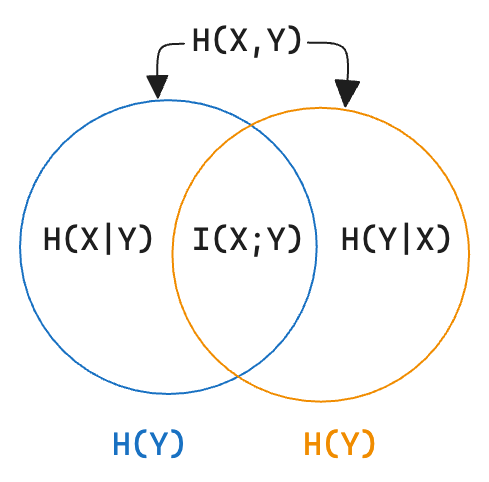
\includegraphics[width=0.3\linewidth]{Figures/venn.png}
    \caption{Relationship between entropy and mutual information.}
    \label{fig:venn}
\end{figure}


\subsection{Chain Rules For Entropy, Relative Entropy, and Mutual Information}

\begin{theorem}[Chain rule for entropy]
    Let $X_1, X_2, \cdots, X_n$ be drawn according to $p(x_1, x_2, \cdots, x_n)$. Then

    \begin{equation}
        \equationgold{
            H(X_1, X_2, \cdots, X_n) = \sum_{i=1}^{n}H(X_i | X_{i-1}, \cdots, X_1)
        }
    \end{equation}
\end{theorem}

\noindent\underline{\textit{Example}}: $H(X_1, X_2, X_3) = H(X_1) + H(X_2 | X_1) + H(X_3 | X_1, X_2)$\\

We now define the conditional mutual information as the reduction in the uncertainty of $X$ due to the knowledge of $Y$ when $Z$ is given.

\begin{definition}[Conditional Mutual Information]
    The conditional mutual information of random variables $X$ and $Y$ given $Z$ is defined by

    \begin{equation}
        I(X; Y | Z) = H(X | Z) - H(X | Y, Z) = \mathbb{E}_{p(x, y, z)}\log\left(\frac{p(X, Y | Z)}{p(X | Z)p(Y | Z)}\right)
    \end{equation}
\end{definition}

\subsection{Jensen's Inequality and its Consequences}

A function $f(x)$ is said to be \hlt{convex} over an interval $(a, b)$ if for every $x_1, x_2 \in (a, b)$ and $0 \leq \lambda \leq 1$,

\begin{equation}
    f(\lambda x_1 + (1 - \lambda)x_2) \leq \lambda f(x_1) + (1 - \lambda)f(x_2)
\end{equation}

A function $f(x)$ is said to be strictly convex if equality holds only if $\lambda = 0$ or $\lambda = 1$. The figure \ref{fig:convex_function} shows an example of each kind of function.

\begin{figure}[ht]
    \centering
    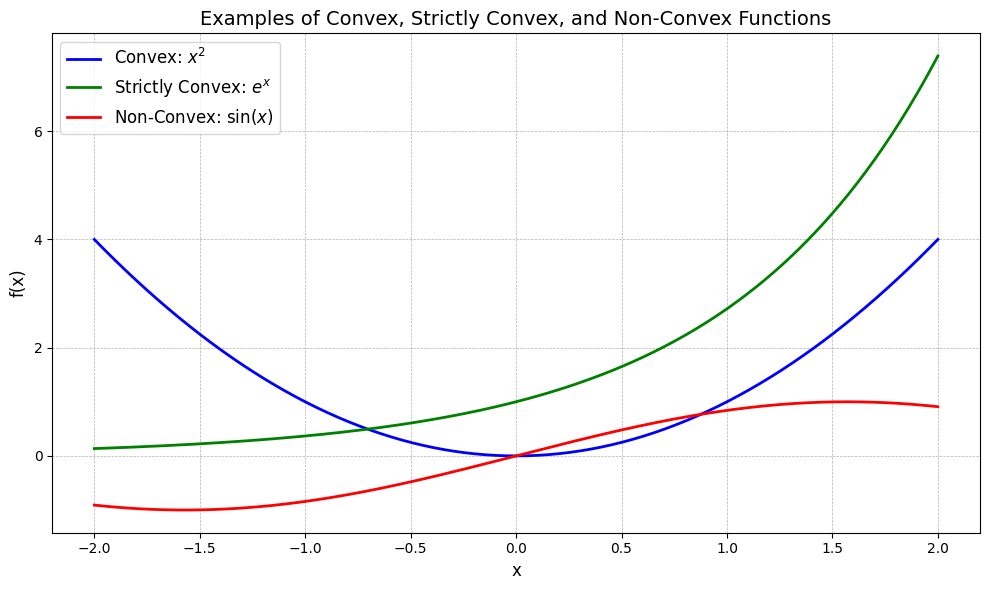
\includegraphics[width=0.5\linewidth]{Figures/convex_function.png}
    \caption{Illustration of a striclty convex, convex, and non convex functions}
    \label{fig:convex_function}
\end{figure}

\begin{theorem}\label{theo:deriv_convex}
    If the function $f$ has a second derivative that is non-negative/positive over an interval, the function is convex/strictly convex over that interval.
\end{theorem}

The figure \ref{fig:convex_derivative} illustrates this theorem. 

\begin{figure}[ht]
    \centering
    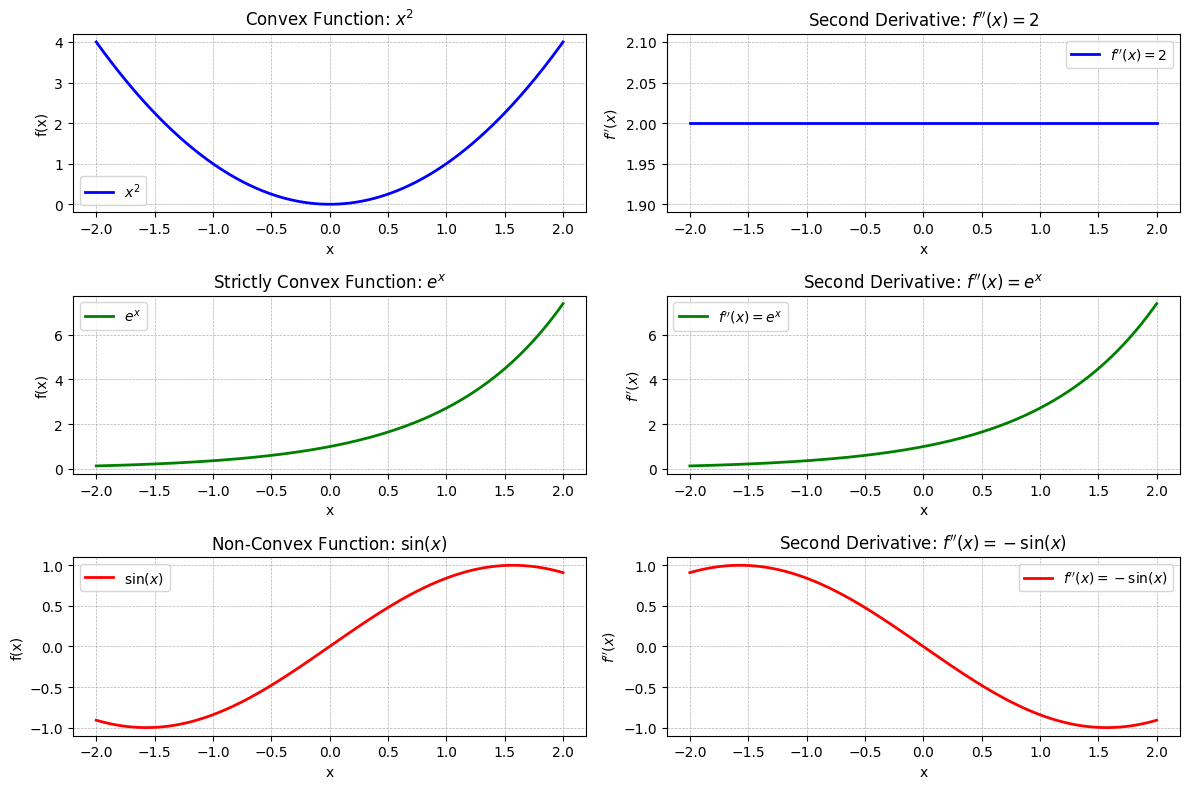
\includegraphics[width=0.7\linewidth]{Figures/convex_derivative.png}
    \caption{Illustration of the second derivative per type of function - Theorem \ref{theo:deriv_convex}.}
    \label{fig:convex_derivative}
\end{figure}

\begin{theorem}[Jensen's Inequality]\label{theo:jensen}
    If $f$ is a \hlt{convex function} and $X$ is a random variable 

    \begin{equation}
        \equationgold{
            \mathbb{E}f[(x)] \geq f(\mathbb{E}[X])
        }
    \end{equation}
\end{theorem}

Moreover, if $f$ is a stricly convex, the equality above implies that $X = EX$ with probability 1 (i.e., $X$ is a constant). Figure \ref{fig:jessen_ine} illustrates some examples of Jensen's Inequality. 

\begin{figure}[ht]
    \centering
    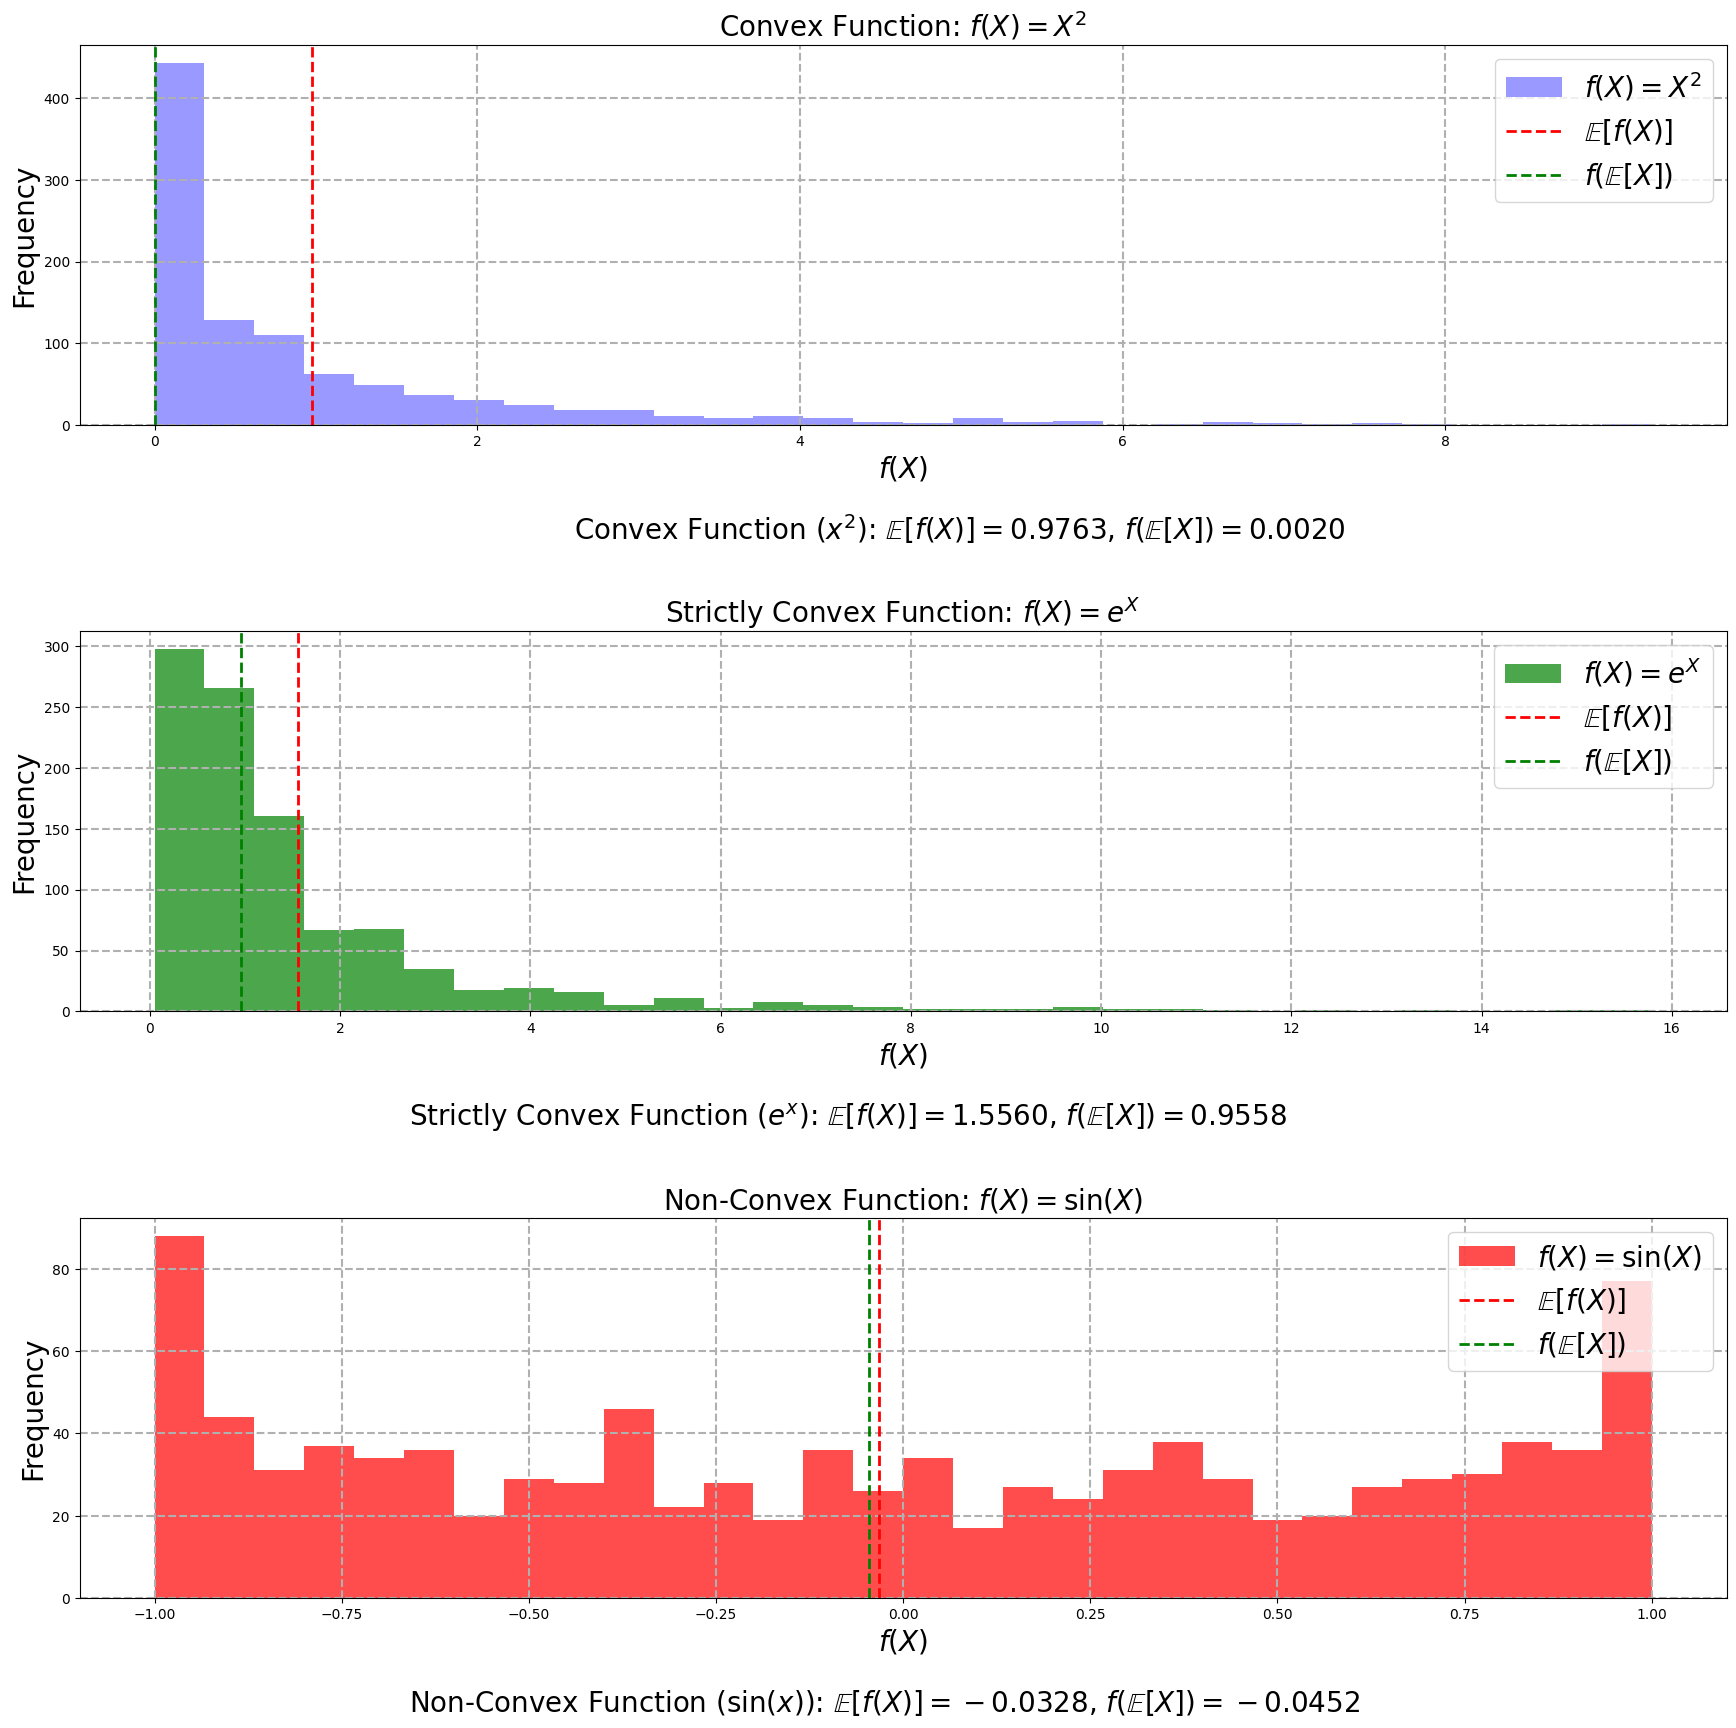
\includegraphics[width=0.7\linewidth]{Figures/jessen_ine.png}
    \caption{Illustration of Jensen's Inequality - Theorem \ref{theo:jensen}.}
    \label{fig:jessen_ine}
\end{figure}

\begin{theorem}[Information Inequality]
    Let $p(x)$, $q(x)$, $x \in \mathcal{X}$ be two probability mass functions. Then
    \begin{equation}
        \equationgold{
            D(p || q) \geq 0
        }
    \end{equation}
    With equality if and only if $p(x) = q(x) \forall x$. This theorem Inequality is also called the \hlt{Divergence Inequality}.
\end{theorem}

\begin{corollary}[Nonnegativity of Mutual Information]
    For any two random variables $X, Y$
    \begin{equation}
        \equationgold{
            I(X; Y) \geq 0
        }
    \end{equation}
    with equality if and only if $X$ and $Y$ are independent.
\end{corollary}

\begin{corollary}
    \begin{equation}        
        D(p(y|x) || q(y|x)) \geq 0
    \end{equation}
    with equality if and only if $p(y|x) = q(y|x)$ for all $y$ and $x$ such that $p(x) > 0$.
\end{corollary}

\begin{corollary}
    \begin{equation}
        \equationgold{
            I(X; Y | Z) \geq 0
        }
    \end{equation}
    with equality if and only if $X$ and $Y$ are conditionally independent given $Z$ that is $X \perp\!\!\!\perp Y \mid Z$.
\end{corollary}

\begin{theorem}
    \begin{equation}
        \equationgold{
            H(X) \leq \log(|H(\mathcal{X})|)
        }
    \end{equation}
    where $|\mathcal{X}|$ denotes the number of elements in the range of $\mathcal{X}$, with equality if and only if $X$  has an uniform distribution over $\mathcal{X}$.
\end{theorem}

\begin{theorem}[Conditioning reduces entropy]
    \begin{equation}
        \equationgold{
            H(X|Y) \leq H(X)
        }
    \end{equation}
    with equality if and only if $X \perp\!\!\!\perp Y$ ($X$ and $Y$ are independent).
\end{theorem}

\begin{theorem}[Independence bound on entropy]\label{theo:ind_bound_entropy}
    Let $X_1, X_2, \cdots, X_n$ be drawn according to $p(x_1, x_2, \cdots, x_n)$. Then 
    \begin{equation}
        \equationgold{
            H(X_1, X_2, \cdots, X_n) \leq \sum_{n}^{i=1}H(X_i)
        }
    \end{equation}
    with equality if and only if $X_i$ are independent.
\end{theorem}

Figure \ref{fig:independence_bound_entropy} shows an example of the independence bound on entropy. 

\begin{figure}[ht]
    \centering
    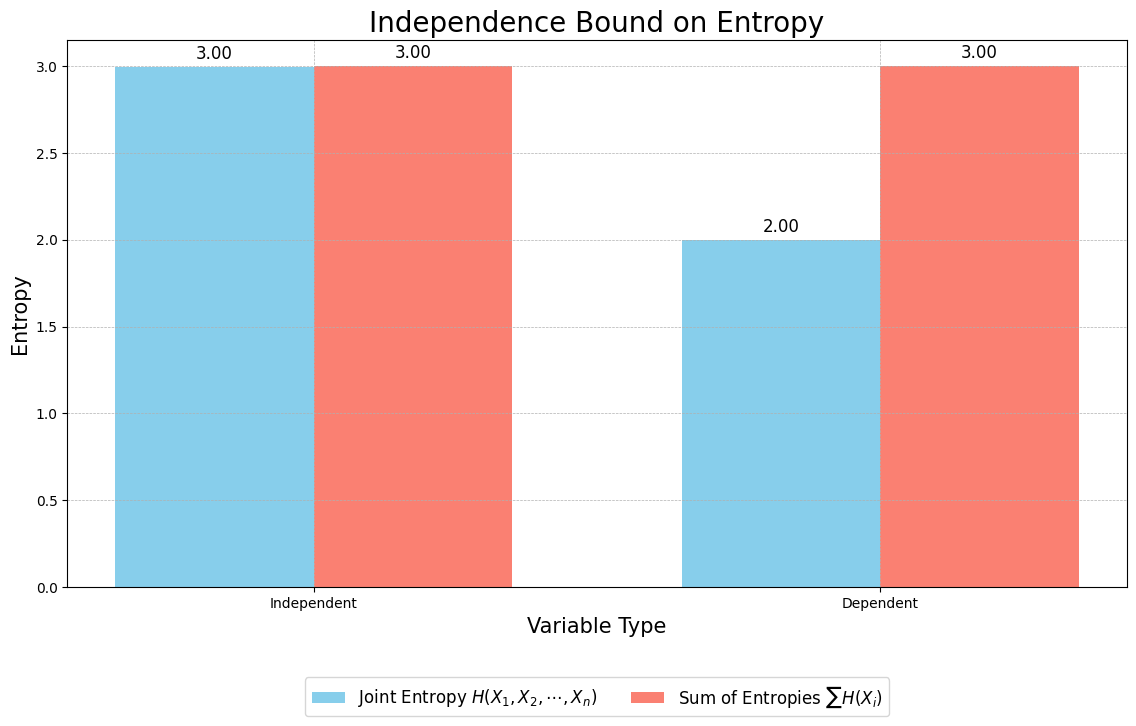
\includegraphics[width=0.7\linewidth]{Figures/independence_bound_entropy.png}
    \caption{Example of the independence bound on entropy - Theorem \ref{theo:ind_bound_entropy}.}
    \label{fig:independence_bound_entropy}
\end{figure}

\begin{lemma}[Fundamental Inequality]\label{lemma:fundamental_inequality}
    For any $a > 0$ 

    \begin{equation}
        \equationgold{
            \ln(a) \leq a - 1
        }
    \end{equation}
    with equality if and only if $a = 1$.
\end{lemma}

Figure \ref{fig:independence_bound_entropy} illustrates the fundamental inequality. 

\begin{figure}[ht]
    \centering
    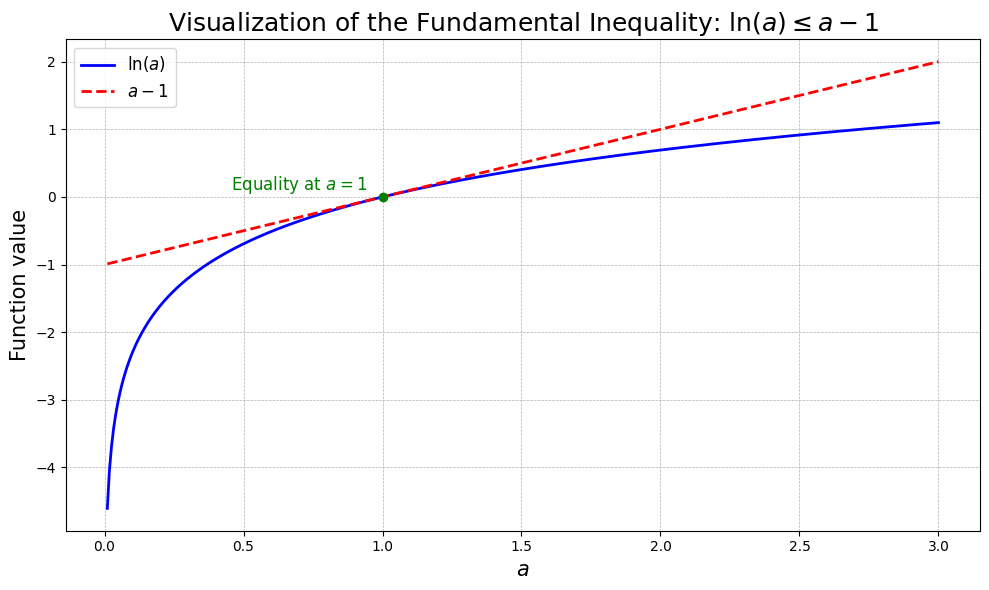
\includegraphics[width=0.7\linewidth]{Figures/fundamental_inequality.png}
    \caption{Example of the fundamental inequality - Lemma \ref{lemma:fundamental_inequality}.}
    \label{fig:fundamental_inequality}
\end{figure}

\begin{theorem}[Concavity of Entropy]
    $H(P)$ is a \hlt{concave} function of $P$.
\end{theorem}

\begin{theorem}
    Let $(X, Y) \sim p(x, y) = p(x)p(y | x)$. The mutual information $I(X; Y)$ is a concave function of $p(x)$ for fixed $p(y|x)$ and a convex function of $p(y|x)$ for fixed $p(x)$.
\end{theorem}

\subsection{Data Processing Inequality}

The data-processing inequality can be used to show that \hlt{no} clever manipulation of the data can \hlt{improve} the inferences that can be made from the data.

\begin{definition}
    Random variables $X, Y, Z$ are said to form a Markov chain in that order (denoted by $X \rightarrow Y \rightarrow Z$) if the conditional distribution of $Z$ depends only on $Y$ and is conditionally independent of $X$. Specifically, $X, Y,$ and $Z$ form a Markov chain $X \rightarrow Y \rightarrow Z$ if the joint probability mass function can be written as 
    \begin{equation}
        p(x, y, z) = p(x)p(y|x)p(z|y)
    \end{equation}
\end{definition}

\begin{theorem}[Data Processing Inequality]\label{theo:data_proc_ineq}
    If $X \rightarrow Y \rightarrow Z$ forms a Markov chain, then 

    \begin{equation}
        \equationgold{
            I(X; Y) \geq I(X; Z) \text{ equivalently } I(X; Z) \geq I(X; Z)
        }
    \end{equation}
    It can also be stated that 
    \begin{equation}
        \equationgold{
            I(X; Y, Z) \geq I(X; Z)
        }
    \end{equation}
\end{theorem}

If the random variables are \hlt{closer} in the Markov Chain, they convey higher mutual information. The figure \ref{fig:data_process_inequality} illustrates such a theorem.

\begin{figure}[ht]
    \centering
    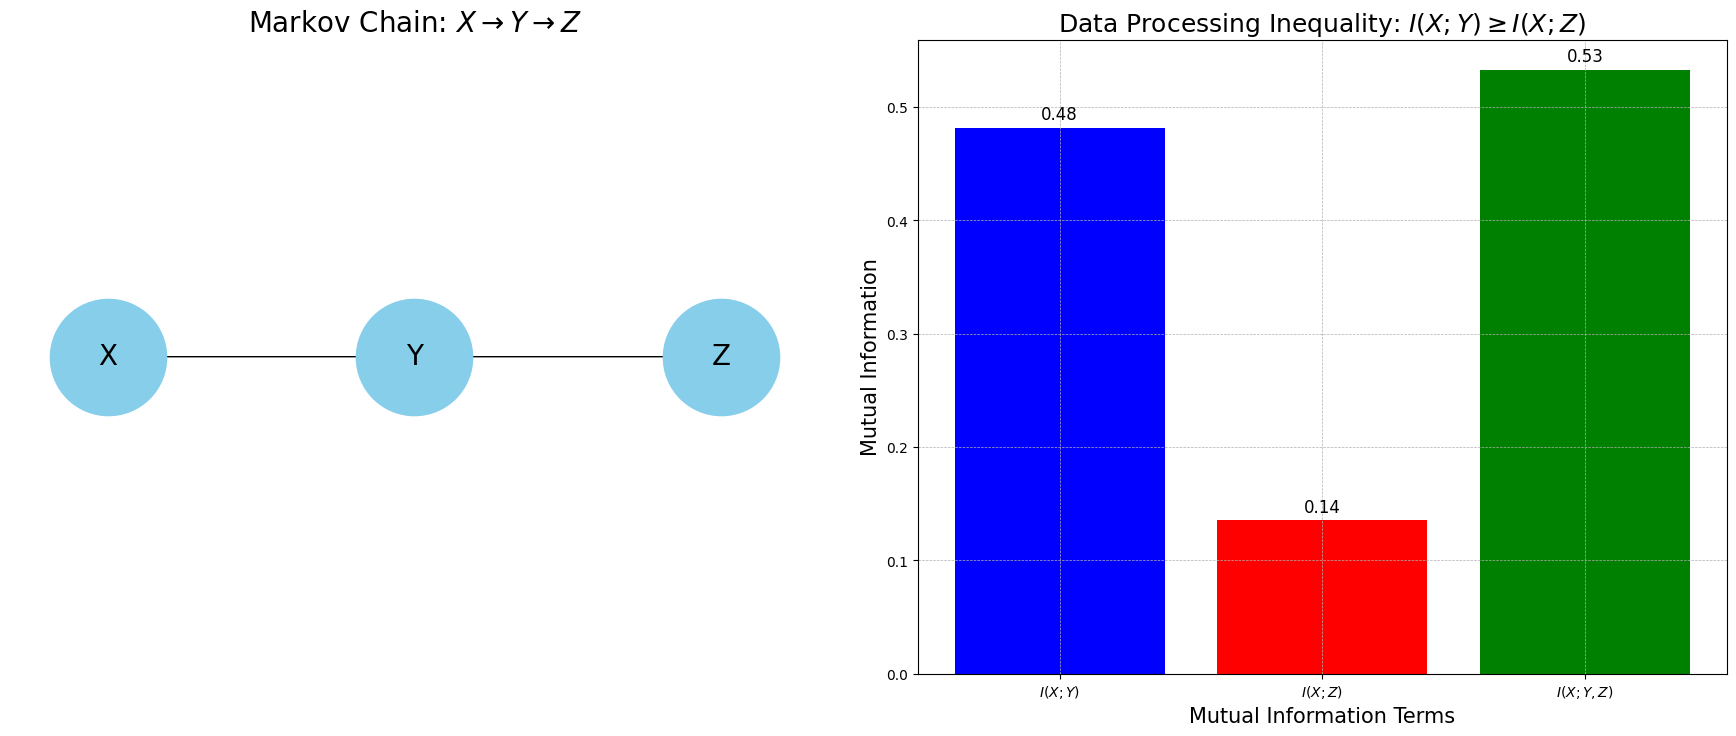
\includegraphics[width=0.7\linewidth]{Figures/dara_process_inequality.png}
    \caption{Example of the data processing inequality - Theorem \ref{theo:data_proc_ineq}.}
    \label{fig:data_process_inequality}
\end{figure}

\subsection{Sufficient Statistics}

\begin{definition}
    A statistic $T(X)$ is said to be a \hlt{sufficient statistic} for $\theta$ if it contains all the information in $X$ about $\theta$.
\end{definition}


Suppose that we have a family of probability mass functions $\{f(x|\theta)\}$ indexed by $\theta$. Let $X$ be a sample from a distribution in the family. Let $T(X)$ be our statistic (function of the sample). Like the sample mean or sample variance. Then \hlt{$\Theta \rightarrow X \rightarrow T(X)$} we have:

$$
I(\theta; X) = I(\theta; T(X)) \text{ for any distribution on } \theta
$$

\noindent due to the data processing inequality we have:

$$
I(\theta; T(X)) \leq I(\theta; X)
$$

A statistic $T(X)$ is called \hlt{sufficient} for $\Theta$ if it contains all the information in $X$ about $\Theta$.

\begin{definition}
    A statistic $T(X)$ is a \hlt{minimal sufficient statistic} relative to $\{ f_\theta(x) \}$ if it's a function of every other sufficient statistic $U$. Interpreting this in terms of the data-processing inequality, this implies that 
    $$
        \Theta \rightarrow T(X) \rightarrow U(X) \rightarrow X
    $$
\end{definition}

\subsection{Fano's Inequality}

Suppose that we know a random variable $Y$ and we wish to guess the value of a correlated random variable $X$. Fano's Inequality relates the probability of error in guessing $X$ to its conditional entropy $H(X | Y)$.

\begin{theorem}[Fano's Inequality]
    For any estimator $\hat{X}$ such that $X \rightarrow Y \rightarrow \hat{X}$, with $P_e = Pr\{ X  \ne \hat{X}\}$

    \begin{equation}
        H(P_e) + P_e \log(|\mathcal{X}|) \geq H(X | \hat{X}) \geq H(X | Y)
    \end{equation}

    This inequality can be weakened to:
    $$
    1 + P_e \log(|\mathcal{X}| \geq H(X|Y))
    $$

    That is
    \begin{equation}
        \equationgold{
            P_e \geq \frac{H(X|Y) - 1}{\log |X|}
        }
    \end{equation}
\end{theorem}

\section{Data Compression}

\begin{quote}
\setlength{\leftskip}{0.25cm} % Adjust the indentation here
$\color{color2}\Longrightarrow$ The following section was written using mainly the book \cite{willey_info_theory} as references.
\end{quote}

\begin{definition}
    A \hlt{source code} $C$ for a random variable $X$ is a mapping from $\mathcal{X}$, the range of $X$, to $\mathcal{D}^*$, the set of finite-length strings of symbols from a $\mathcal{D}$-any alphabet. Let $C(x)$ denote the codeword corresponding to $x$ and let $l(x)$ denote the length of $C(x)$
\end{definition}

\begin{definition}
    The \hlt{expected length} $L(C)$ of a source code $C(x)$ for a random variable $X$ with probability mass function $p(x)$ is given by 

    \begin{equation}
        \equationgold{
            L(C) = \sum_{x \in \mathcal{X}} p(x)l(x)
        }
    \end{equation}
\end{definition}

\noindent \underline{\textit{Example}}: Suppose we have a random variable $ X $ with the following probability mass function:

$$
p(X) = \begin{cases}
0.4 & \text{if } X = A \\
0.3 & \text{if } X = B \\
0.2 & \text{if } X = C \\
0.1 & \text{if } X = D
\end{cases}
$$

Let's consider a source code $ C $ with the following codewords:

$$
C(A) = 0, \quad C(B) = 10, \quad C(C) = 110, \quad C(D) = 111
$$

The lengths of the codewords are:

$$
l(A) = 1, \quad l(B) = 2, \quad l(C) = 3, \quad l(D) = 3
$$

The entropy $ H(X) $ of the random variable $ X $ is given by:

$$
H(X) = - \sum_{x \in \mathcal{X}} p(x) \lg p(x)
$$

Substituting the given probabilities:

$$
H(X) = - [0.4 \lg 0.4 + 0.3 \lg 0.3 + 0.2 \lg 0.2 + 0.1 \lg 0.1] \implies H(X) = 1.8464 \text{bits}
$$

The expected length $ L(C) $ of the source code $ C $ is given by:

$$
L(C) = \sum_{x \in \mathcal{X}} p(x) l(x)
$$

Substituting the given probabilities and codeword lengths:

$$
L(C) = 0.4 \cdot 1 + 0.3 \cdot 2 + 0.2 \cdot 3 + 0.1 \cdot 3 \implies L(C) = 1.9 \text{bits}
$$

\subsection{Nonsingular Code}

\begin{definition}
    A \hlt{nonsingular code} is a code in which different source symbols are mapped to distinct codewords. Formally, a code $C$ is nonsingular if $C(x_i) \neq C(x_j)$ for all $x_i \neq x_j$ in the source alphabet $\mathcal{X}$.
\end{definition}

\noindent \underline{\textit{Example}}: Consider the source alphabet $\mathcal{X} = \{A, B, C\}$ and the codebook $C = \{00, 01, 10\}$. This code is nonsingular because each symbol maps to a unique codeword:
$$
C(A) = 00, \quad C(B) = 01, \quad C(C) = 10
$$

\subsection{Uniquely Decodable Code}

\begin{definition}
    A \hlt{uniquely decodable code} is a code in which every sequence of codewords maps to at most one sequence of source symbols. In other words, no two different sequences of source symbols result in the same sequence of codewords.
\end{definition}

\noindent \underline{\textit{Example}}: Consider the source alphabet $\mathcal{X} = \{A, B\}$ and the codebook $C = \{0, 10\}$. This code is uniquely decodable because any sequence of codewords can be uniquely parsed:

$$
\text{Code sequence: } 010 \quad \text{decodes to: } AB
$$
$$
\text{Code sequence: } 1010 \quad \text{decodes to: } BB
$$

\subsection{Prefix Code}

\begin{definition}
    A \hlt{prefix code} (or prefix-free code) is a code in which no codeword is a prefix of any other codeword. This property ensures that the code can be instantly decoded without the need for lookahead.
\end{definition}

\noindent \underline{\textit{Example}}: Consider the source alphabet $\mathcal{X} = \{A, B, C\}$ and the codebook $C = \{0, 10, 110\}$. This code is a prefix code because no codeword is a prefix of any other.

\subsection{Instantaneous Code}

\begin{definition}
    A \hlt{instantaneous code} is a code in which each codeword can be decoded immediately upon receipt of the final symbol in the codeword. All prefix codes are instantaneous codes.
\end{definition}

\noindent \underline{\textit{Example}}: Using the same example as the prefix code: consider the source alphabet $\mathcal{X} = \{A, B, C\}$ and the codebook $C = \{0, 10, 110\}$. This code is also an instantaneous code. The code is instantaneous because once we receive a codeword, we can immediately decode it without waiting for any additional symbols.\\

\noindent \underline{\textit{Example}}: Consider the source alphabet $\mathcal{X} = \{A, B, C\}$ and the codebook $C = \{0, 01, 011\}$. This code is non-instantaneous because the codeword for $ B $ is a prefix of the codeword for $ C $.

\subsection{Kraft Inequality}

We wish to construct instaneous codes for minimum expected length to describe a given source. 

\begin{theorem}[Kraft Inequality]
    For any instaneous code (prefix code) over an alphabet of size $D$, the codeword lengths $l_1, l_2, \cdots, l_m$ must satisfy the Inequality
    \begin{equation}
        \sum_{i} D^{l_i} \leq 1
    \end{equation}
\end{theorem}

Conversely, given a set of codewords lengths that satisfy this inequality there exists an instantneous code with these word lengths. The idea of Kraft Inequality can be understood through the table \ref{tab:symbol_code_budget} shown in the online class of \cite{mackay_youtube_playlist}.

\section{The Mathematics of Neural Networks}

\subsection{Notation}

Let's just give a big picture overview with the notations we'll use:

\begin{itemize}
    \item $m$ -  size of train set
    \item $n$ - amount of input variables 
    \item $L$ - amount of layers in the Neural Network
    \item $l$ - specific layer
    \item $w^l$ - the weight $w$ of the specific layer $l$
    \item $b^l$ - bias $b$ for specific layer $l$
    \item $x_i$ - single input variable
\end{itemize}

\subsection{Big Picture}

A Neural Network is just a big "fancy" function made up of a lot of smaller functions. The output is often a scalar it can be a continous number or a category (classification) which depending of the set of inputs $\{ x_1, x_2, \cdots, x_n \}$ of the neural network.

We can think this problem as a big calculus problem where we are always trying to minimize our cost. In some sense it's all about minimization and about calculating $\frac{\partial Cost}{\partial w}$, in other words, we're always trying to find the influence of weights into our cost function. How much twickling the weights make the cost change. In a more general view, we should algo consider the bias in this influence as well. Basically, by changing the weights and biases how much the final cost is impacted. 

\subsection{Matrix Calculation Review}

Let's see on example using the equations shown below:

$$ F(x, y) = x^2 + \cos y $$

\noindent where 

$$ \frac{\partial F}{\partial x} = 2x \quad \frac{\partial F}{\partial y} = -\sin y $$

\subsubsection{Gradients}

With that in mind we can remind ourselved of the \textbf{gradient} function ($\mathcal{R}^n \rightarrow \mathcal{R}^1$) which is defined as

$$
\nabla F(x, y) = \begin{bmatrix}
    \frac{\partial F(x, y)}{\partial x} \\
    \frac{\partial F(x, y)}{\partial y}
\end{bmatrix}
$$

Thus, for our example

$$
\nabla F(x, y) = \begin{bmatrix}
    2x \\
    - \sin y
\end{bmatrix}
$$

\subsubsection{Jacobian}

Let's now talk about \textbf{Jacobians} ($\mathcal{R}^n \rightarrow \mathcal{R}^m$) let's imaginge the function 

$$
F(x, y) : \mathcal{R}^2 = \begin{bmatrix}
2x + y^3 \\
e^y - 13x
\end{bmatrix}.
$$

\noindent where we can say that $f_1 = 2x + y^2$ and $f_2 = e^y - 13x$. Now, let's take the partial derivatives for each function

$$ \frac{\partial f_1}{\partial x} = 2 \quad \frac{\partial f_1}{\partial y} = 3y^2 $$
$$ \frac{\partial f_2}{\partial x} = -13 \quad \frac{\partial f_2}{\partial y} = e^y $$

Let's now define the Jacobian 

$$
J(F(x, y)) = \begin{bmatrix}
\frac{\partial f_1}{\partial x} & \frac{\partial f_1}{\partial y} \\
&\\
\frac{\partial f_2}{\partial x} & \frac{\partial f_2}{\partial y}
\end{bmatrix}.
$$

We could write this using the $\nabla$ symbol for gradient as shown below

$$
J(F(x, y)) = \begin{bmatrix}
\nabla f_1^T \\
\\
\nabla f_2^T
\end{bmatrix}.
$$

For our function this results in 

$$
J(F(x, y)) = \begin{bmatrix}
2 & 3y^2 \\
-13 & e^y
\end{bmatrix}
$$

\subsubsection{Jacobian chain rule}

We know that the chain rule is defined as 

$$ \frac{\partial y}{\partial x} = \frac{\partial y}{\partial u} \frac{\partial u}{\partial x}$$

\textit{\underline{example}}: for the function $y = \sin(x^2)$ by assigning $u = x^2$ we have

$$ 
   \frac{\partial y}{\partial x} = \frac{\partial y}{\partial u} \frac{\partial u}{\partial x} = \frac{\partial \sin(u)}{\partial u} \frac{\partial x^2}{\partial x} = \cos(u) 2x
$$

Finally, 

$$ 
   \frac{\partial y}{\partial x} = 2x\cos(x^2)
$$

Let's now see this process for a Jacobian matrix. That is, 

$$
F(x, y) = \begin{bmatrix}
\sin(x^2 + y) \\
\ln(y^3)
\end{bmatrix}
$$

Then our intermediate functions $u$ can be defined as 

$$
\bm{u} = \begin{bmatrix}
    u_1\\
    u_2
\end{bmatrix} = \begin{bmatrix}
    x^2 + y \\
    y^3
\end{bmatrix} \quad \text{ and } \quad
F(x, y) = \bm{f} = \begin{bmatrix}
    f_1\\
    f_2
\end{bmatrix} = \begin{bmatrix}
    \sin(u_1) \\
    \ln(u_2)
    \end{bmatrix}
$$

Let's now calculate the partial derivatives

$$
\frac{\partial \bm{u}}{\partial \bm{x}} = \begin{bmatrix}
    \frac{\partial u_1}{\partial x} & \frac{\partial u_1}{\partial y} \\
    &\\
    \frac{\partial u_2}{\partial x} & \frac{\partial u_2}{\partial y}
\end{bmatrix} = \begin{bmatrix}
    2x & 1 \\
    0 & 3y^2
\end{bmatrix} \quad \text{ and } \quad
\frac{\partial \bm{f}}{\partial \bm{u}} = \begin{bmatrix}
    \frac{\partial f_1}{\partial u_1} & \frac{\partial f_2}{\partial u_1} \\
    &\\
    \frac{\partial f_2}{\partial u_1} & \frac{\partial f_2}{\partial u_2}
\end{bmatrix} = \begin{bmatrix}
    \cos(u_1) & 0 \\
    0 & \frac{1}{u_2}
\end{bmatrix}
$$

Since we know that $\frac{\partial y}{\partial x} = \frac{\partial y}{\partial u} \frac{\partial u}{\partial x}$ we have

$$
\frac{\partial \bm{f}}{\partial \bm{x}} = \frac{\partial \bm{f}}{\partial \bm{u}} \frac{\partial \bm{u}}{\partial \bm{x}}
$$

$$
\frac{\partial \bm{f}}{\partial \bm{x}} = \begin{bmatrix}
    \cos(u_1) && 0 \\
    0 && \frac{1}{u_2} 
\end{bmatrix} 
\begin{bmatrix}
    2x && 1 \\
    0 && 3y^2
\end{bmatrix} = \begin{bmatrix}
    2x\cos(u_1) & \cos(u_1) \\
    0 & \frac{3y^2}{u_2} 
\end{bmatrix} = \begin{bmatrix}
    2x\cos(x^2 + y) & \cos(x^2 + y) \\
    0 & \frac{3y^2}{y^3} 
\end{bmatrix}
$$

Which finally retrieve us, 

$$
    \frac{\partial \bm{f}}{\partial \bm{x}} = \begin{bmatrix}
        2x\cos(x^2 + y) & \cos(x^2 + y) \\
        0 & \frac{3}{y} 
    \end{bmatrix} 
$$

Look how the matrix above is giving us the information about how much influence each variable has. In other words, if we change our variable $x$ our function $f_1 = \sin(x^2 + y)$ will be affected by $\frac{\partial f_1}{\partial x} = 2x\cos(x^2 + y)$ which is the element (1, 1) in our matrix $\frac{\partial \bm{f}}{\partial \bm{x}}$ and the same happens for the rest of the matrix elements.

\subsection{Forward Propagation}

\subsubsection{The Neuron Function}

We can see the output of a neuron in mathematical terms as

$$
    f(\bm{x}; \bm{w}, b) = \sum^n_{i=1}x_i w_i + b
$$

$$
    z = \sigma( f(\bm{x}; \bm{w}, b) )
$$

\noindent note that $\sum^n_{i=1}x_i w_i$ is basically a scalar and $\sigma$ is the \textit{sigmoid} activation function. However, the basic idea of how the inputs of a neuron are computed is that they are a dot product of their respective weights. That is,

$$
\begin{bmatrix}
    x_1 & x_2 & \cdots & x_n
\end{bmatrix}\begin{bmatrix}
    w_1 \\
    w_2 \\
    \vdots\\
    w_n
\end{bmatrix} = x_1 w_1 + x_2 w_2 + \cdots + x_n w_n
$$


Hence, we can rewrite our expression as 

$$
    f(\bm{x}; \bm{w}, b) = \bm{x}^T \bm{w} + b
$$

$$
    z = \sigma(f(\bm{x}; \bm{w}, b))
$$

\subsubsection{Layer of NN}

When we represent a neural network we should always think in matrices since basically all our operations will be based on matrix multiplication and summation. For instance, image we consider the following weight matrix

$$
\bm{W} = \begin{bmatrix}
    w^1_{1, 1} & w^1_{1, 2}\\
    w^1_{2, 1} & w^1_{2, 2}
\end{bmatrix} = \begin{bmatrix}
    5 & 2\\
    3 & 6
\end{bmatrix}
$$

Basically this weight matrix is retrieving us the schematic for a neural network. As we can see on the image below. 
Then, using this matrix notation we can get the output per layer, assuming the input is $x_1 = 10$ and $x_2 = 20$ and the bias is $b = 6$ we thus have 

$$
a^1 = \bm{W}\bm{X} + b = \begin{bmatrix}
    5 & 2\\
    3 & 6
\end{bmatrix} \begin{bmatrix}
    10 \\
    20
\end{bmatrix} = \begin{bmatrix}
    90 \\
    150
\end{bmatrix} + 6 = \begin{bmatrix}
    96 \\
    156
\end{bmatrix}
$$

Then we can compute our output $z$ by applying sigmoid function 

$$
z = \sigma(\bm{W}\bm{X} + b) = \begin{bmatrix}
    96 \\
    156
\end{bmatrix}
$$

Basically, we can understand the feedforward as a combination of layers as shown below.

$$
    a_0 = \sigma(W^1 a_0 + b^1)
$$

$$
    a_1 = \sigma(W^2 a_1 + b^2)
$$

$$
    a_n = \sigma(W^{n+1} a_n + b^n)
$$

\section{General Exercises and Solutions}

The following exercises are some of the questions I've encountered during the course of Information Theory from The Chinese University of Hong Kong. The reference book for those exercises is the following: \href{https://link.springer.com/book/10.1007/978-0-387-79234-7}{Information Theory and Network Coding}.

\noindent \textbf{Note:} The following solutions are unofficial and should not be considered as an official guide.

\subsection{Chapter 2}

\subsection*{Question 1}
Let $X$ and $Y$ be random variables with alphabets $\mathcal{X} = \mathcal{Y} = \{1, 2, 3, 4, 5\}$ and joint distribution $p(x, y)$ given by:

$$
p(x, y) = \frac{1}{25}
\begin{bmatrix}
1 & 1 & 1 & 1 & 1 \\
2 & 1 & 2 & 0 & 0 \\
0 & 1 & 1 & 1 & 1 \\
0 & 3 & 0 & 2 & 0 \\
0 & 0 & 1 & 1 & 3 \\
\end{bmatrix}
$$

Calculate $H(X), H(Y), H(X|Y), H(Y|X),$ and $I(X;Y)$.

\textbf{Solution:}

1. Calculate Marginal Probabilities:

$$
p_X(x) = \sum_{y} p(x, y), \quad p_Y(y) = \sum_{x} p(x, y)
$$

2. Calculate Entropies:

$$
H(X) = -\sum_{x} p_X(x) \log p_X(x), \quad H(Y) = -\sum_{y} p_Y(y) \log p_Y(y)
$$

3. Conditional Entropies:

$$
H(X|Y) = -\sum_{x, y} p(x, y) \log \frac{p(x, y)}{p_Y(y)}, \quad H(Y|X) = -\sum_{x, y} p(x, y) \log \frac{p(x, y)}{p_X(x)}
$$

4. Mutual Information:

$$
I(X; Y) = H(X) + H(Y) - H(X, Y)
$$

$$
H(X, Y) = -\sum_{x, y} p(x, y) \log p(x, y)
$$

\subsection*{Question 2}
Prove Propositions 2.8, 2.9, 2.19, 2.21, and 2.22.

\textbf{Proposition 2.8}
$X_1 \to X_2 \to \cdots \to X_n$ forms a Markov chain if and only if
$$
X_1 \to X_2 \to X_3, \quad (X_1, X_2) \to X_3 \to X_4, \quad \ldots, \quad (X_1, X_2, \ldots, X_{n-2}) \to X_{n-1} \to X_n
$$
form Markov chains.

\textbf{Proof:}
To show that a sequence of random variables $X_1, X_2, \ldots, X_n$ forms a Markov chain, we need to show that the conditional probability of $X_{k+1}$ depends only on $X_k$ for each $k$. This can be expressed as:
$$
p(X_{k+1} | X_1, X_2, \ldots, X_k) = p(X_{k+1} | X_k)
$$
for all $k \in \{1, 2, \ldots, n-1\}$.

If we define the joint probability distribution of $X_1, X_2, \ldots, X_n$ as $p(x_1, x_2, \ldots, x_n)$, then by the chain rule of probability, we have:
$$
p(x_1, x_2, \ldots, x_n) = p(x_1) \cdot p(x_2|x_1) \cdots p(x_n|x_1, \ldots, x_{n-1})
$$
If $X_1 \to X_2 \to \cdots \to X_n$ forms a Markov chain, then:
$$
p(x_{k+1} | x_1, \ldots, x_k) = p(x_{k+1} | x_k) \quad \forall k
$$
which means that the sequence $(X_1, X_2, \ldots, X_{k}) \to X_{k+1} \to X_{k+2}$ forms a Markov chain. This completes the proof.

\textbf{Proposition 2.9}
$X_1 \to X_2 \to \cdots \to X_n$ forms a Markov chain if and only if
$$
p(x_1, x_2, \cdots, x_n) = f_1(x_1, x_2) f_2(x_2, x_3) \cdots f_{n-1}(x_{n-1}, x_n)
$$
for all $x_1, x_2, \cdots, x_n$ such that $p(x_2), p(x_3), \cdots, p(x_{n-1}) > 0$.

\textbf{Proof:}
Suppose $X_1 \to X_2 \to \cdots \to X_n$ forms a Markov chain. By definition, this means:
$$
p(X_{k+1} | X_1, \ldots, X_k) = p(X_{k+1} | X_k) \quad \forall k
$$
Using the chain rule, the joint distribution can be written as:
$$
p(x_1, x_2, \ldots, x_n) = p(x_1) \cdot p(x_2|x_1) \cdot p(x_3|x_2) \cdots p(x_n|x_{n-1})
$$
Thus, the joint probability can be factored into terms involving only consecutive pairs, which proves the forward direction.

For the converse, if the joint distribution can be factored as:
$$
p(x_1, x_2, \ldots, x_n) = f_1(x_1, x_2) f_2(x_2, x_3) \cdots f_{n-1}(x_{n-1}, x_n)
$$
it follows that $p(X_{k+1}| X_1, \ldots, X_k) = f_{k}(X_k, X_{k+1})$ depends only on $X_k$. Thus, the sequence forms a Markov chain.

\textbf{Proposition 2.19}
$$
I(X; Y) = H(X) - H(X|Y), \quad I(X; Y) = H(Y) - H(Y|X)
$$
and
$$
I(X; Y) = H(X) + H(Y) - H(X, Y)
$$
provided that all the entropies and conditional entropies are finite.

\textbf{Proof:}
The mutual information between two random variables $X$ and $Y$ is defined as:
$$
I(X; Y) = \sum_{x, y} p(x, y) \log \frac{p(x, y)}{p(x)p(y)}
$$
By manipulating the logarithmic terms, we obtain:
$$
I(X; Y) = H(X) - H(X|Y) = H(Y) - H(Y|X) = H(X) + H(Y) - H(X, Y)
$$
This completes the proof.

\textbf{Proposition 2.21}
The mutual information between a random variable $X$ and itself conditioning on a random variable $Z$ is equal to the conditional entropy of $X$ given $Z$, i.e.,
$$
I(X; X|Z) = H(X|Z).
$$

\textbf{Proof:}
By definition, the conditional mutual information $I(X; X|Z)$ is given by:
$$
I(X; X|Z) = H(X|Z) - H(X|X, Z)
$$
Since $H(X|X, Z) = 0$, we have:
$$
I(X; X|Z) = H(X|Z)
$$
This completes the proof.

\textbf{Proposition 2.22}
$$
I(X; Y|Z) = H(X|Z) - H(X|Y, Z), \quad I(X; Y|Z) = H(Y|Z) - H(Y|X, Z)
$$
and

$$
I(X; Y|Z) = H(X|Z) + H(Y|Z) - H(X, Y|Z)
$$

provided that all the conditional entropies are finite.

\textbf{Proof:}
The mutual information between $X$ and $Y$ given $Z$ is defined as:

$$
I(X; Y|Z) = \sum_{x, y, z} p(x, y, z) \log \frac{p(x, y | z)}{p(x | z)p(y | z)}
$$

By expanding the logarithmic terms, we obtain:

$$
I(X; Y|Z) = H(X|Z) - H(X|Y, Z) = H(Y|Z) - H(Y|X, Z) = H(X|Z) + H(Y|Z) - H(X, Y|Z)
$$

This completes the proof.

\subsection*{Question 3}
Give an example which shows that pairwise independence does not imply mutual independence.

\textbf{Solution:}

Consider three random variables $X, Y, Z$ defined as follows:
- $X, Y,$ and $Z$ are pairwise independent if $p(X, Y) = p(X)p(Y)$, $p(Y, Z) = p(Y)p(Z)$, and $p(X, Z) = p(X)p(Z)$.
- However, the triplet $(X, Y, Z)$ is not mutually independent because $p(X, Y, Z) \neq p(X)p(Y)p(Z)$.

\subsection*{Question 4} Verify that $p(x, y, z)$ as defined in Definition 2.4 is a probability distribution. You should exclude all the zero probability masses from the summation carefully.

\textbf{Definition 2.4} (Conditional Independence). For random variables $X, Y,$ and $Z$, $X$ is independent of $Z$ conditioning on $Y$, denoted by $X \perp Z | Y$, if:

$$
p(x, y, z)p(y) = p(x, y)p(y, z) \quad \text{for all } x, y, \, \text{and} \, z, \quad (2.3)
$$

or equivalently,

$$
p(x, y, z) = 
\begin{cases}
\frac{p(x, y)p(y, z)}{p(y)} & \text{if } p(y) > 0, \\
0 & \text{otherwise}.
\end{cases} \quad (2.4)
$$

\textbf{Solution:}

To verify that $p(x, y, z)$ is a probability distribution, we need to show that the sum of $p(x, y, z)$ over all possible values of $x, y,$ and $z$ is equal to 1, i.e.,

$$
\sum_{x, y, z} p(x, y, z) = 1.
$$

Using Definition 2.4, we have:

$$
p(x, y, z) = 
\begin{cases}
\frac{p(x, y)p(y, z)}{p(y)} & \text{if } p(y) > 0, \\
0 & \text{otherwise}.
\end{cases}
$$

Thus, we can compute the sum over all non-zero terms:

$$
\sum_{x, y, z} p(x, y, z) = \sum_{y : p(y) > 0} \sum_{x} \sum_{z} \frac{p(x, y)p(y, z)}{p(y)}.
$$

Since $p(y) > 0$, we can separate the summation:

$$
\sum_{y : p(y) > 0} \frac{1}{p(y)} \left( \sum_{x} p(x, y) \right) \left( \sum_{z} p(y, z) \right).
$$

Note that $\sum_{x} p(x, y) = p(y)$ and $\sum_{z} p(y, z) = p(y)$, so we have:

$$
\sum_{y : p(y) > 0} \frac{1}{p(y)} \cdot p(y) \cdot p(y) = \sum_{y : p(y) > 0} p(y) = 1.
$$

Thus, the sum of $p(x, y, z)$ over all $x, y,$ and $z$ is equal to 1, which confirms that $p(x, y, z)$ is a valid probability distribution.

\subsection*{Question 5}
\textbf{Linearity of Expectation} It is well-known that expectation is linear, i.e., $E[f(X) + g(Y)] = E[f(X)] + E[g(Y)]$, where the summation in an expectation is taken over the corresponding alphabet. However, we adopt in information theory the convention that the summation in an expectation is taken over the corresponding support. Justify carefully the linearity of expectation under this convention.

\textbf{Solution:}

By the definition of expectation, we have:

$$
E[f(X) + g(Y)] = \sum_{x, y} p(x, y) \cdot (f(x) + g(y))
$$

Splitting the summation:

$$
E[f(X)] = \sum_{x} p_X(x) \cdot f(x), \quad E[g(Y)] = \sum_{y} p_Y(y) \cdot g(y)
$$

Hence, we can show that:

$$
E[f(X) + g(Y)] = E[f(X)] + E[g(Y)]
$$

\subsection*{Question 11}
Prove that $ H(p) $ is concave in $ p $, i.e., for $ 0 \leq \lambda \leq 1 $ and $ \bar{\lambda} = 1 - \lambda $:

$$
\lambda H(p_1) + \bar{\lambda} H(p_2) \leq H(\lambda p_1 + \bar{\lambda} p_2).
$$

\textbf{Solution:}

The entropy function $ H(p) $ for a binary random variable can be defined as:

$$
H(p) = -p \log p - (1-p) \log (1-p),
$$

where $ 0 \leq p \leq 1 $.

To prove that $ H(p) $ is concave, we need to show that for any $ 0 \leq \lambda \leq 1 $ and $ p_1, p_2 \in [0,1] $:
$$
\lambda H(p_1) + (1-\lambda) H(p_2) \leq H(\lambda p_1 + (1-\lambda)p_2).
$$

The function $ H(p) $ is concave if the second derivative $ H''(p) $ is non-positive for all $ p $. Let's compute the second derivative of $ H(p) $:

First, compute the first derivative:
$$
H'(p) = -\log p + \log (1-p).
$$

Now, compute the second derivative:
$$
H''(p) = -\frac{1}{p} - \frac{1}{1-p}.
$$
Simplify it further:
$$
H''(p) = -\left(\frac{1}{p(1-p)}\right).
$$
Since $ p(1-p) > 0 $ for $ 0 < p < 1 $, $ H''(p) $ is negative, implying that $ H(p) $ is concave.

Therefore, the inequality $ \lambda H(p_1) + \bar{\lambda} H(p_2) \leq H(\lambda p_1 + \bar{\lambda} p_2) $ holds, proving the concavity of $ H(p) $.


\subsection*{Question 12}
Let $ (X,Y) \sim p(x,y) = p(x)p(y|x) $.

\textbf{Part (a):} Prove that for fixed $ p(x) $, $ I(X;Y) $ is a convex functional of $ p(y|x) $.

\textbf{Solution:}

The mutual information $ I(X;Y) $ is given by:
$$
I(X;Y) = \sum_{x,y} p(x) p(y|x) \log \frac{p(y|x)}{p(y)},
$$
where $ p(y) = \sum_{x} p(x) p(y|x) $.

For fixed $ p(x) $, $ I(X;Y) $ is convex in $ p(y|x) $. This is because the function $ p \log p $ is convex for $ p \geq 0 $. To see this, consider two conditional distributions $ p_1(y|x) $ and $ p_2(y|x) $ and a mixing parameter $ 0 \leq \lambda \leq 1 $.

The convexity of mutual information implies:
$$
I(X; \lambda p_1(y|x) + (1-\lambda) p_2(y|x)) \leq \lambda I(X; p_1(y|x)) + (1-\lambda) I(X; p_2(y|x)).
$$

This convexity arises because the log function is concave, and a sum of convex functions weighted by probabilities is convex.

\textbf{Part (b):} Prove that for fixed $ p(y|x) $, $ I(X;Y) $ is a concave functional of $ p(x) $.

\textbf{Solution:}

For fixed $ p(y|x) $, mutual information $ I(X;Y) $ can be written as:
$$
I(X;Y) = H(Y) - H(Y|X),
$$
where $ H(Y) $ is the entropy of $ Y $ and $ H(Y|X) $ is the conditional entropy.

$ H(Y|X) $ is linear in $ p(x) $, and $ H(Y) $ is a concave function of $ p(x) $. The concavity of $ I(X;Y) $ in $ p(x) $ follows from the fact that the entropy function $ H(Y) $ is concave in $ p(x) $, and mutual information is the difference between the concave function $ H(Y) $ and the linear function $ H(Y|X) $.

Therefore, for any two distributions $ p_1(x) $ and $ p_2(x) $ and any $ 0 \leq \lambda \leq 1 $, we have:
$$
I(\lambda p_1(x) + (1-\lambda)p_2(x); Y) \geq \lambda I(p_1(x); Y) + (1-\lambda)I(p_2(x); Y).
$$

\subsection*{Question 15}

Let $ X $ be a function of $ Y $. Prove that $ H(X) \leq H(Y) $. Interpret this result.

\textbf{Solution:}

Let $ X = f(Y) $, where $ f $ is a deterministic function. The entropy $ H(Y) $ represents the uncertainty in $ Y $, and $ H(X) $ represents the uncertainty in $ X $. Since $ X $ is determined by $ Y $, knowing $ Y $ gives complete knowledge of $ X $. Therefore, the uncertainty (entropy) of $ X $ cannot exceed that of $ Y $:

$$
H(X) \leq H(Y).
$$

This result can also be understood by noting that if $ X $ is a deterministic function of $ Y $, there is no additional randomness in $ X $ given $ Y $. The interpretation is that a function of a random variable cannot have more uncertainty (entropy) than the original variable itself.

\subsection*{Question 16}

Prove that for any $ n \geq 2 $,

$$
H(X_1, X_2, \dots, X_n) \geq \sum_{i=1}^{n} H(X_i | X_j, j \neq i).
$$

\textbf{Solution:}

The strong subadditivity of entropy states that the joint entropy of a set of random variables is greater than or equal to the sum of the conditional entropies. 

For $ n = 2 $, this inequality becomes:
$$
H(X_1, X_2) \geq H(X_1 | X_2) + H(X_2 | X_1).
$$
This is equivalent to the fact that mutual information $ I(X_1; X_2) \geq 0 $.

For $ n \geq 3 $, the inequality can be proved by induction:

\textbf{Base Case:} For $ n = 3 $,

$$
H(X_1, X_2, X_3) \geq H(X_1 | X_2, X_3) + H(X_2 | X_1, X_3) + H(X_3 | X_1, X_2).
$$

This follows directly from the chain rule of entropy:

$$
H(X_1, X_2, X_3) = H(X_1) + H(X_2 | X_1) + H(X_3 | X_1, X_2).
$$

The right-hand side is the sum of the individual entropies minus the mutual information terms, which are non-negative.

\textbf{Inductive Step:} Assume the inequality holds for $ n-1 $ random variables. For $ n $ variables, the inequality follows similarly by applying the chain rule of entropy and summing conditional entropies. Thus, the strong subadditivity holds for any $ n \geq 2 $.

\subsection*{Question 17}
Prove that

$$
H(X_1, X_2) + H(X_2, X_3) + H(X_1, X_3) \geq 2 H(X_1, X_2, X_3).
$$

\noindent \textbf{Hint:} Sum the identities

$$
H(X_1, X_2, X_3) = H(X_j, j \neq i) + H(X_i | X_j, j \neq i)
$$

\noindent for $ i = 1, 2, 3 $ and apply the result in Problem 16.

\textbf{Solution:}

Using the identities provided and the result from Problem 16, we can prove this inequality. Consider the three identities:

$$
H(X_1, X_2, X_3) = H(X_2, X_3) + H(X_1 | X_2, X_3),
$$
$$
H(X_1, X_2, X_3) = H(X_1, X_3) + H(X_2 | X_1, X_3),
$$
$$
H(X_1, X_2, X_3) = H(X_1, X_2) + H(X_3 | X_1, X_2).
$$

Adding these identities gives:

$$
3H(X_1, X_2, X_3) = H(X_1, X_2) + H(X_2, X_3) + H(X_1, X_3) + H(X_1 | X_2, X_3) + H(X_2 | X_1, X_3) + H(X_3 | X_1, X_2).
$$

Now, apply the result from Problem 16, which states:

$$
H(X_1, X_2, X_3) \geq H(X_1 | X_2, X_3) + H(X_2 | X_1, X_3) + H(X_3 | X_1, X_2).
$$

Thus, the inequality simplifies to:

$$
2H(X_1, X_2, X_3) \leq H(X_1, X_2) + H(X_2, X_3) + H(X_1, X_3).
$$

This completes the proof.

\subsection*{Question 18}

For a subset $ \alpha $ of $ N_n = \{1, 2, \dots, n\} $, denote $ (X_i, i \in \alpha) $ by $ X_\alpha $. For $ 1 \leq k \leq n $, let

$$
H_k = \frac{1}{{n \choose k}} \sum_{\alpha:|\alpha|=k} \frac{H(X_\alpha)}{k}.
$$

Here $ H_k $ is interpreted as the average entropy per random variable when $ k $ random variables are taken from $ X_1, X_2, \dots, X_n $ at a time. Prove that

$$
H_1 \geq H_2 \geq \dots \geq H_n.
$$

\textbf{Solution:}

This sequence of inequalities is known as Han's inequality for entropy. To prove this, we note that:

\begin{enumerate}
    \item $ H_k $ is a normalized sum of entropies, where $ H(X_\alpha) $ represents the joint entropy of the $ k $ variables $ X_\alpha $.
    \item The key observation is that adding more random variables tends to increase the entropy (since entropy is a measure of uncertainty or information). However, because $ H_k $ is normalized by dividing by $ k $, the average entropy per variable decreases as $ k $ increases.
    \item More formally, since $ H(X_1, \dots, X_k) \leq H(X_1, \dots, X_{k+1}) $, normalizing by $ k $ and $ k+1 $ respectively, we get:
    $$
    \frac{H(X_1, \dots, X_k)}{k} \geq \frac{H(X_1, \dots, X_{k+1})}{k+1}.
    $$

    Summing over all subsets $ \alpha $ of size $ k $ and $ k+1 $, and normalizing by the binomial coefficients, we obtain:

    $$
    H_k \geq H_{k+1}.
    $$

    Thus, $ H_1 \geq H_2 \geq \dots \geq H_n $.
\end{enumerate}

\subsection*{Question 20}
Prove the divergence inequality by using the log-sum inequality.

\textbf{Solution:}

The divergence or Kullback-Leibler divergence between two probability distributions $ P $ and $ Q $ over a finite set $ X $ is defined as:

$$
D(P \| Q) = \sum_{x \in X} P(x) \log \frac{P(x)}{Q(x)}.
$$

To prove that $ D(P \| Q) \geq 0 $, we use the log-sum inequality. The log-sum inequality states that for non-negative numbers $ a_i $ and $ b_i $, $ i = 1, \dots, n $, we have:

$$
\sum_{i=1}^{n} a_i \log \frac{a_i}{b_i} \geq \left(\sum_{i=1}^{n} a_i\right) \log \frac{\sum_{i=1}^{n} a_i}{\sum_{i=1}^{n} b_i},
$$

with equality if and only if $ \frac{a_i}{b_i} $ is the same for all $ i $.

Now, let $ a_i = P(x_i) $ and $ b_i = Q(x_i) $, where $ \sum_{i=1}^{n} P(x_i) = 1 $ and $ \sum_{i=1}^{n} Q(x_i) = 1 $. Applying the log-sum inequality, we get:

$$
\sum_{x \in X} P(x) \log \frac{P(x)}{Q(x)} \geq 1 \cdot \log 1 = 0,
$$

with equality if and only if $ P(x) = Q(x) $ for all $ x $. Thus, $ D(P \| Q) \geq 0 $.


\subsection{Chapter 3}

\subsection*{Question 9}
\textbf{(a) Statement:} Prove that under the constraint that $ X \to Y \to Z $ forms a Markov chain, $ X \perp Z | Y $ and $ X \perp Z $ imply $ X \perp Y $.

\textbf{Solution:}

Given that $ X \to Y \to Z $ forms a Markov chain, we have:
$$
p(z|x,y) = p(z|y).
$$
If $ X \perp Z | Y $, then $ p(z|x,y) = p(z|y) $. Since $ p(z|x,y) = p(z|y) $, and $ p(z|x) = p(z) $ when $ X \perp Z $, we must have $ X \perp Y $. Thus, $ X \perp Y $ is implied.

\textbf{(b) Statement:} Prove that the implication in (a) continues to be valid without the Markov chain constraint.

\textbf{Solution:}

Without the Markov chain constraint, $ X \perp Z | Y $ and $ X \perp Z $ do not necessarily imply $ X \perp Y $. A counterexample can be constructed where $ X $ and $ Y $ are dependent, but $ X \perp Z | Y $ and $ X \perp Z $ hold. Thus, the implication does not hold without the Markov chain constraint.

\subsection*{Question 10}
\textbf{(a) Statement:} Show that $ Y \perp Z | T $ does not imply $ Y \perp Z | (X,T) $ by giving a counterexample.

\textbf{Solution:}

Consider a scenario where $ Y $, $ Z $, and $ T $ are independent, but $ X $ introduces a dependency between $ Y $ and $ Z $. For example, let $ X $ be a common cause of $ Y $ and $ Z $. Then $ Y \perp Z | T $ holds, but $ Y $ and $ Z $ may not be independent given $ X $ and $ T $.

\textbf{(b) Statement:} Prove that $ Y \perp Z | T $ implies $ Y \perp Z | (X,T) $ conditioning on $ X \to Y \to Z \to T $.

\textbf{Solution:}

If $ X \to Y \to Z \to T $ forms a chain, the mutual information $ I(Y; Z | T) = 0 $ implies $ I(Y; Z | X, T) = 0 $. This follows from the fact that adding $ X $ does not introduce new dependencies between $ Y $ and $ Z $ given $ T $.

\subsection*{Question 11}
\textbf{(a)} Let $ X \to Y \to (Z,T) $ form a Markov chain. Prove that $ I(X; Z) + I(X; T) \leq I(X; Y) + I(Z; T) $.

\textbf{Solution:}

We use the chain rule of mutual information:

$$
I(X; Z, T) = I(X; Z) + I(X; T | Z),
I(X; Y, Z, T) = I(X; Y) + I(X; Z | Y) + I(X; T | Y, Z).
$$

Given that $ X \to Y \to (Z,T) $ forms a Markov chain, we have:

$$
I(X; Z | Y) = 0 \quad \text{and} \quad I(X; T | Y, Z) = 0.
$$

Thus:

$$
I(X; Z) + I(X; T) \leq I(X; Y) + I(Z; T).
$$

\textbf{(b) Statement:} Let $ X \to Y \to Z \to T $ form a Markov chain. Determine which of the following inequalities always hold:
\begin{itemize}
    \item[(i)] $ I(X; T) + I(Y; Z) \geq I(X; Z) + I(Y; T) $.
    \item[(ii)] $ I(X; T) + I(Y; Z) \geq I(X; Y) + I(Z; T) $.
    \item[(iii)] $ I(X; Y) + I(Z; T) \geq I(X; Z) + I(Y; T) $.
\end{itemize}

\textbf{Solution:}

(i) $ I(X; T) + I(Y; Z) \geq I(X; Z) + I(Y; T) $ is not always true.

(ii) $ I(X; T) + I(Y; Z) \geq I(X; Y) + I(Z; T) $ holds due to the chain rule and properties of Markov chains.

(iii) $ I(X; Y) + I(Z; T) \geq I(X; Z) + I(Y; T) $ is also true, as it is derived from the conditional mutual information.

\subsection*{Question 14}
Prove that for random variables $ X $, $ Y $, $ Z $, and $ T $:

$$
\begin{aligned}
Y \perp Z | X \quad &\Rightarrow \quad Y \perp Z, \\
(X, Y) \perp T | Z \quad &\Rightarrow \quad Y \perp Z, \\
X \perp T \quad &\Rightarrow \quad Y \perp Z, \\
Y \perp Z | T \quad &\Rightarrow \quad X \perp T.
\end{aligned}
$$

\textbf{Solution:}

This problem asks to use the information diagram and properties of conditional independence. Since each implication corresponds to a specific setup in the diagram, using the properties of conditional mutual information and the definition of Markov chains helps establish these relationships.

\subsection*{Question 15}
Prove that:

$$
\begin{aligned}
X \perp Y, \\
X \perp Y | (Z, T), \\
Z \perp T | X, \\
Z \perp T | Y,
\end{aligned}
$$
is equivalent to:
$$
\begin{aligned}
Z \perp T, \\
Z \perp T | (X, Y), \\
X \perp Y | Z, \\
X \perp Y | T.
\end{aligned}
$$

\textbf{Solution:}

We need to show that each statement on the left is equivalent to a corresponding statement on the right using properties of conditional independence and mutual information. This equivalence can be proven by examining the conditional independence structure and applying the symmetry of mutual information.

\subsection{Chapter 4}

\subsection*{Question 1}
Construct a binary Huffman code for the distribution $\{0.25, 0.05, 0.1, 0.13, 0.2, 0.12, 0.08, 0.07\}$.

\textbf{Solution:}

To construct a binary Huffman code we need to:

\begin{enumerate}
    \item Sort the probabilities in ascending order: $\{0.05, 0.07, 0.08, 0.1, 0.12, 0.13, 0.2, 0.25\}$.
    \item Merge the two smallest probabilities, $\{0.05, 0.07\}$ to get a new probability of $0.12$.
    \item Repeat this process until all symbols are combined into a single probability.
\end{enumerate}

The final Huffman code tree and the corresponding binary codes for each probability are:

\begin{table}[h!]
    \centering
    \begin{tabular}{|c|c|c|}
        \hline
        \textbf{Symbol} & \textbf{Probability} & \textbf{Code} \\
        \hline
        \{0.25\} & 0.25 & 0 \\
        \{0.2\} & 0.2 & 10 \\
        \{0.12\} & 0.12 & 110 \\
        \{0.13\} & 0.13 & 1110 \\
        \{0.1\} & 0.1 & 11110 \\
        \{0.08\} & 0.08 & 111110 \\
        \{0.07\} & 0.07 & 1111110 \\
        \{0.05\} & 0.05 & 1111111 \\
        \hline
    \end{tabular}
    \caption{Huffman Code Table for Given Probabilities}
    \label{tab:huffman_code}
\end{table}

\subsection*{Question 2}
Construct a ternary Huffman code for the source distribution in Problem 1.

\textbf{Solution:}

In a ternary Huffman code, we merge the three smallest probabilities instead of two:

\begin{itemize}
    \item Initial probabilities: $\{0.05, 0.07, 0.08, 0.1, 0.12, 0.13, 0.2, 0.25\}$.
    \item Merge $\{0.05, 0.07, 0.08\}$ to get a new probability of $0.2$.
    \item Repeat the process until only one probability remains.
\end{itemize}

The final ternary codes are:

\begin{table}[h!]
    \centering
    \begin{tabular}{|c|c|c|}
        \hline
        \textbf{Symbol} & \textbf{Probability} & \textbf{Code} \\
        \hline
        \{0.25\} & 0.25 & 0 \\
        \{0.2\} & 0.2 & 10 \\
        \{0.13\} & 0.13 & 20 \\
        \{0.12\} & 0.12 & 21 \\
        \{0.1\} & 0.1 & 22 \\
        \{0.08\} & 0.08 & 100 \\
        \{0.07\} & 0.07 & 101 \\
        \{0.05\} & 0.05 & 102 \\
        \hline
    \end{tabular}
    \caption{Ternary Huffman Code Table for Given Probabilities}
    \label{tab:ternary_huffman_code}
\end{table}



\subsection*{Question 3}
Show that a Huffman code is an optimal uniquely decodable code for a given source distribution.

\textbf{Solution:}

A uniquely decodable code is a code in which no codeword is a prefix of any other codeword. To prove that a Huffman code is optimal, we can show that the average code length is minimized. This is achieved by the construction of the Huffman algorithm, which greedily merges the least probable symbols.

Let $l_i$ be the length of codeword for symbol $i$ with probability $p_i$. The average code length is:

$$
L = \sum_{i} p_i l_i.
$$

Huffman coding ensures that $L$ is minimized, satisfying the Kraft inequality:

$$
\sum_{i} 2^{-l_i} \leq 1.
$$

\subsection*{Question 5}
Prove directly that the codeword lengths of a prefix code satisfy the Kraft inequality without using Theorem 4.4.

\textbf{Solution:}

The Kraft inequality states that for a prefix code with codeword lengths $ l_1, l_2, \dots, l_n $, we must have:
$$
\sum_{i=1}^{n} 2^{-l_i} \leq 1.
$$
A prefix code means no codeword is a prefix of another. We can prove the inequality by constructing a binary tree and showing that the sum of the probabilities corresponding to the codewords at each level cannot exceed 1.

\subsection*{Question 7}
Show that a suffix code is uniquely decodable.

\textbf{Solution:}

A suffix code is a code where no codeword is a suffix of another codeword. We can prove unique decodability by constructing the decoding tree backward (starting from the leaves) and showing that each sequence of bits leads to a unique codeword.

\subsection*{Question 9}

Construct a binary prefix code with codeword lengths $ l_1 \leq l_2 \leq \dots \leq l_m $ as follows:
For each $ 1 \leq k \leq m $, the codeword with length $ l_k $ is chosen independently from the set of all $ 2^{l_k} $ possible binary strings with length $ l_k $ according to the uniform distribution. Let $ P_m(\text{good}) $ be the probability that the code so constructed is a prefix code.

\textbf{(a) Solution:}

For $ P_2(\text{good}) = (1 - 2^{-l_1})^+ $, where:
$$
(x)^+ = \begin{cases}
x & \text{if } x \geq 0, \\
0 & \text{if } x < 0.
\end{cases}
$$

\textbf{(b) Solution:}

Prove by induction on $ m $ that:
$$
P_m(\text{good}) = \prod_{k=1}^{m} \left(1 - \sum_{j=1}^{k-1} 2^{-l_j}\right)^+.
$$
This can be done by showing that the inclusion of an additional codeword maintains the prefix condition and that the product form correctly accounts for the independence of the choices.

\textbf{(c) Solution:}

Observe that there exists a prefix code with codeword lengths $ l_1, l_2, \dots, l_m $ if and only if $ P_m(\text{good}) > 0 $. Show that $ P_m(\text{good}) > 0 $ is equivalent to the Kraft inequality. Using this random coding method, one can derive the Kraft inequality without knowing the inequality ahead of time.

\subsection{Chapter 5}

\subsection*{Question 1}
Show that for any $\epsilon > 0$, $W_{[X]_{\epsilon}}^n$ is nonempty for sufficiently large $n$.

\textbf{Solution:}

Let $W_{[X]_{\epsilon}}^n$ denote the $\epsilon$-typical set. We need to show that the probability of $W_{[X]_{\epsilon}}^n$ approaches 1 as $n \to \infty$. By the Law of Large Numbers, for any $\epsilon > 0$, the probability that a sequence belongs to $W_{[X]_{\epsilon}}^n$ increases as $n$ becomes large. Thus:

$$
\lim_{n \to \infty} \Pr(W_{[X]_{\epsilon}}^n) = 1.
$$

\subsection*{Question 2}
Prove that $P_e \to 1$ as $n \to \infty$ even if we are allowed to use a general block code.

\textbf{Solution:}

Using the source coding theorem, we have that the error probability for a block code with a finite alphabet converges to 1 as $n \to \infty$ for any code that does not satisfy the source coding rate:

$$
R > H(X).
$$

Thus, $P_e \to 1$ as $n \to \infty$.

\subsection*{Question 5}
(a) Show that for any $x \in \mathcal{X}^n$,

$$
- \frac{1}{n} \log p(x) = D(q_x \| p) + H(q_x).
$$

\textbf{Proof:}

By the definition of the empirical distribution $q_x$, we have:

$$
p(x) = \prod_{i=1}^n p(x_i) = 2^{-n H(q_x)} \cdot 2^{-n D(q_x \| p)}.
$$

Taking the logarithm and dividing by $-n$, we get:

$$
- \frac{1}{n} \log p(x) = D(q_x \| p) + H(q_x).
$$

(b) Show that for any $\epsilon > 0$, the weakly typical set $W_{[X]_{\epsilon}}^n$ is the set of sequences $x \in \mathcal{X}^n$ such that:

$$
|D(q_x \| p) + H(q_x) - H(p)| \leq \epsilon.
$$

\textbf{Proof:}

By the asymptotic equipartition property (AEP), for large $n$, $D(q_x \| p) \approx 0$ and $H(q_x) \approx H(p)$. Thus, for $\epsilon > 0$, the set of sequences that satisfy this condition is the weakly typical set.

\newpage
\fontsize{8}{9}\selectfont
\bibliography{ResearchPaperBib}

\clearpage

\end{document}